\documentclass[12pt,a4paper]{article}

% ============================================
% PAQUETES ESENCIALES
% ============================================
\usepackage[utf8]{inputenc}        
\usepackage[T1]{fontenc}             
\usepackage[spanish,es-tabla]{babel}  

\usepackage{times} 
\usepackage{geometry}
\usepackage{setspace}
\usepackage{graphicx}
\usepackage{titlesec}
\usepackage{fancyhdr}
\usepackage{enumitem}
\usepackage{hyperref}
\usepackage{tabularx}
\usepackage{booktabs}
\usepackage{longtable}
\usepackage{multirow}
\usepackage{pdflscape}
\usepackage{fmtcount}
\usepackage{comment}
\usepackage{float}
\usepackage{caption}
\usepackage{siunitx}
\usepackage{ragged2e}
\usepackage{array}
\usepackage[table]{xcolor}
\usepackage{colortbl} 

% ============================================
% CONFIGURACIÓN DE URLS Y MÁRGENES DE HOJA
% ============================================
\usepackage{url}
\Urlmuskip=0mu plus 1mu 
\makeatletter
\g@addto@macro{\UrlBreaks}{\do\/\do\-\do\.\do\=\do\_\do\?\do\&\do\%}
\makeatother

\geometry{
	a4paper,
	top=2.5cm,
	bottom=2.5cm,
	left=3cm,
	right=2cm
}
\setstretch{1.5}

% ============================================
% PAQUETE TOCLOFT Y CONFIGURACIÓN DE ÍNDICES (APA 7)
% ============================================
\usepackage{tocloft}
% Corrección de colisión horizontal del número romano VII
\setlength{\cftsecnumwidth}{3.2em} 

% Formateo para incluir la palabra "Tabla X" en la lista de tablas
\renewcommand{\cfttabpresnum}{\textbf{Tabla }} 
\setlength{\cfttabnumwidth}{4.5em}             
\renewcommand{\cfttabaftersnumb}{\hspace{0.1em}} 

% Formateo para incluir la palabra "Figura X" en la lista de figuras
\renewcommand{\cftfigpresnum}{\textbf{Figura }} 
\setlength{\cftfignumwidth}{4.8em}             
\renewcommand{\cftfigaftersnumb}{\hspace{0.1em}} 

% ============================================
% CONFIGURACIÓN DE HIPERVÍNCULOS
% ============================================
\hypersetup{
	colorlinks=true,
	linkcolor=black,
	citecolor=black,
	urlcolor=blue,
	pdfencoding=auto
}

% ============================================
% CONFIGURACIÓN DE TÍTULOS
% ============================================
\titleformat{\section}{\normalfont\fontsize{12}{15}\bfseries\uppercase}{\thesection}{1em}{}
\titleformat{\subsection}{\normalfont\fontsize{12}{15}\bfseries}{\thesubsection}{1em}{}
\titleformat{\subsubsection}{\normalfont\fontsize{12}{15}\bfseries}{\thesubsubsection}{1em}{}

% ============================================
% ENCABEZADOS Y PIES DE PÁGINA
% ============================================
\pagestyle{fancy}
\fancyhf{}
\fancyfoot[C]{\thepage}
\renewcommand{\headrulewidth}{0pt}

% ============================================
% CONFIGURACIÓN DE TABLAS SEGÚN APA 7
% ============================================
\captionsetup[table]{
	format=plain,
	labelformat=simple,
	labelsep=newline,
	labelfont=bf,
	textfont=it,
	justification=raggedright,
	singlelinecheck=false,
	position=top
}

% ============================================
% INFORMACIÓN INSTITUCIONAL DEL DOCUMENTO
% ============================================
\newcommand{\universidadLinea}{UNIVERSIDAD NACIONAL}
\newcommand{\universidadLineaDos}{SANTIAGO ANTÚNEZ DE MAYOLO}
\newcommand{\facultad}{FACULTAD DE CIENCIAS}
\newcommand{\escuela}{ESCUELA PROFESIONAL DE INGENIERÍA DE SISTEMAS E INFORMÁTICA}
\newcommand{\tituloTesis}{PROTOTIPO DE SMART PARKING SYSTEM APLICANDO TECNOLOGÍAS EMERGENTES DE INTERNET OF THINGS, ARTIFICIAL INTELLIGENCE Y CLOUD COMPUTING DEL EJE SMART MOBILITY PARA SMART CITY EN HUARAZ - ANCASH, 2025}
\newcommand{\autor}{EDWIN YONER FLORES RUPAY}
\newcommand{\asesor}{FRANZ MARTÍN VILLANUEVA COCHACHIN} 
\newcommand{\ciudad}{Huaraz}
\newcommand{\anio}{2026}

% ============================================
% CUERPO PRINCIPAL DEL DOCUMENTO
% ============================================
\begin{document}
	
	\pagenumbering{gobble}
	
	% ============================================
	% CARÁTULA O PORTADA
	% ============================================
	\begin{titlepage}
		\centering
		\setstretch{1.2}
		{\large\bfseries \universidadLinea \par}
		{\large\bfseries \universidadLineaDos \par}
		\vspace{0.5cm}
		{\large\bfseries \facultad \par}
		\vspace{0.5cm}
		{\large\bfseries \escuela \par}
		\vspace{0.8cm}
		
		
\includegraphics[width=0.25\textwidth]{logo_unasam.png}
		\vspace{0.8cm}
		
		{\Large\bfseries PROYECTO DE TESIS \par}
		\vspace{0.75cm}
		
		{\normalsize\bfseries \tituloTesis \par}
		\vfill
		
		{\large PRESENTADO POR: \par}
		\vspace{0.3cm}
		{\large Bachiller: \autor \par}
		\vspace{1cm}
		
		{\large ASESOR: \par}
		\vspace{0.3cm}
		{\large Maestro: \asesor \par}
		\vfill
		
		{\large HUARAZ - PERÚ \par}
		{\large \anio \par}
	\end{titlepage}
	
	% ============================================
	% SECCIÓN DE ÍNDICES PRELIMINARES
	% ============================================
	\clearpage
	\pagenumbering{Roman}
	\setcounter{page}{1}
	
	% 1. Índice General (Contenido)
	\renewcommand{\contentsname}{CONTENIDO}
	\tableofcontents
	\clearpage
	
	% 2. Índice de Tablas (Lista de tablas con prefijo automático)
	\renewcommand{\listtablename}{ÍNDICE DE TABLAS}
	\phantomsection % <-- CREA EL ANCLA CORRECTA DE HIPERVÍNCULO AQUÍ
	\addcontentsline{toc}{section}{\listtablename}
	\listoftables
	\clearpage
	
	% 3. Índice de Figuras (Lista de figuras con prefijo automático)
	\renewcommand{\listfigurename}{ÍNDICE DE FIGURAS}
	\phantomsection % <-- CREA EL ANCLA CORRECTA DE HIPERVÍNCULO AQUÍ
	\addcontentsline{toc}{section}{\listfigurename}
	\listoffigures
	\clearpage
	
% ============================================
% PRIMERA PARTE: DATOS GENERALES
% ============================================
\phantomsection % <-- CREA EL ANCLA CORRECTA PARA ESTE TÍTULO SIN NÚMERO
\section*{PRIMERA PARTE: DATOS GENERALES}
\addcontentsline{toc}{section}{PRIMERA PARTE: DATOS GENERALES}

\subsection*{1. TÍTULO}
\addcontentsline{toc}{subsection}{1. Título}
\tituloTesis

\subsection*{2. AUTOR}
\addcontentsline{toc}{subsection}{2. Autor}
\begin{itemize}[leftmargin=*]
    \item \textbf{Apellidos y nombres:} Flores Rupay Edwin Yoner
\end{itemize}

\subsection*{3. ASESOR}
\addcontentsline{toc}{subsection}{3. Asesor}
\begin{itemize}[leftmargin=*]
    \item \textbf{Apellidos y nombres:} Villanueva Cochachin Franz Martín
    \item \textbf{Grado académico:} Maestro en ciencias e ingeniería con mención en auditoría y seguridad informática
    \item \textbf{Título profesional:} Ingeniero Electrónico
    \item \textbf{Dirección laboral:} Universidad Nacional Santiago Antúnez De Mayolo\\
    Av. Universitaria S/N – Barrio Shancayan - Distrito de Independencia
\end{itemize}

\begin{comment}
\subsection*{4. LÍNEA Y SUBLÍNEA DE INVESTIGACIÓN}
\addcontentsline{toc}{subsection}{4. Línea y sublínea de investigación}
\begin{itemize}[leftmargin=*]
    \item \textbf{Línea de investigación:} Energía Renovable E Innovación Tecnológica
    \item \textbf{Sublínea de investigación:} Ciencia De Datos E Ingeniería Para La Inteligencia Artificial
\end{itemize}
\end{comment}

\subsection*{4. LÍNEA Y SUBLÍNEA DE INVESTIGACIÓN}
\addcontentsline{toc}{subsection}{4. Línea y sublínea de investigación}
\begin{itemize}[leftmargin=*]
	\item \textbf{Área de investigación:} Ingeniería y Tecnología
	\item \textbf{Línea de investigación:} Energía Renovable e Innovación Tecnológica
	\item \textbf{Sublíneas de investigación:} 
	\begin{itemize}
		\item Ciencia de datos e ingeniería para la inteligencia artificial
		\item Sistema de información e ingeniería de software
		\item Seguridad, negocios electrónicos, Cloud computing y gestión de bases de datos
		\item Redes de telecomunicaciones, sistemas electrónicos, digitales y de control
	\end{itemize}
\end{itemize}

\subsection*{5. TIPO DE INVESTIGACIÓN}
\addcontentsline{toc}{subsection}{5. Tipo de investigación}

\subsubsection*{5.1. De acuerdo a la orientación}
\addcontentsline{toc}{subsubsection}{5.1. De acuerdo a la orientación}
\textbf{Aplicada:} La investigación está orientada a desarrollar un prototipo destinado a contribuir a la solución de problemas relacionados con la gestión de parqueos en la ciudad de Huaraz, contribuyendo al desarrollo de ciudades inteligentes en la región.

\subsubsection*{5.2. De acuerdo a la técnica de contrastación}
\addcontentsline{toc}{subsubsection}{5.2. De acuerdo a la técnica de contrastación} 
\textbf{Explicativa:} Se utilizará experimentación mediante el desarrollo e implementación de un prototipo que integra tecnologías Internet of Things, Artificial Intelligence y Cloud Computing. Los datos serán obtenidos por observación de fenómenos condicionados por el investigador, evaluando variables de rendimiento, eficiencia y usabilidad en escenarios controlados de gestión de parqueos.

\subsection*{6. RÉGIMEN DE INVESTIGACIÓN}
\addcontentsline{toc}{subsection}{6. Régimen de investigación}

\textbf{Orientada:} El tema de investigación se encuentra alineado con las líneas de investigación de la Facultad de Ciencias, específicamente dentro del área de \textbf{Ingeniería y Tecnología}, línea de investigación \textbf{Energía Renovable e Innovación Tecnológica}, aprobadas según el documento "Líneas de Investigación de la UNASAM" del Vicerrectorado de Investigación (2021).

El proyecto integra las cuatro sublíneas de investigación mediante una arquitectura tecnológica articulada. La sublínea 30: \textit{Redes de telecomunicaciones, sistemas electrónicos, digitales y de control}, sustenta las tecnologías de Internet of Things. A partir de los datos obtenidos, la sublínea 27: \textit{Ciencia de datos e ingeniería para la inteligencia artificial}, permite aplicar técnicas de Artificial intelligence. Posteriormente, la sublínea 29: \textit{Seguridad, negocios electrónicos, Cloud computing y gestión de bases de datos}, proporciona el soporte para la gestión de los datos mediante servicios de Cloud Computing. Finalmente, la sublínea 28: \textit{Sistema de información e ingeniería de software}, permite articular estos componentes mediante la arquitectura de software, los servicios backend, frontend y móvil que conforman el prototipo. De esta manera, las cuatro sublíneas se complementan entre sí para sustentar el desarrollo integral del prototipo de Smart Parking.

\subsection*{7. LOCALIDAD E INSTITUCIÓN DONDE SE DESARROLLARÁ EL PROYECTO}
\addcontentsline{toc}{subsection}{7. Localidad e institución}
\begin{itemize}[leftmargin=*]
    \item \textbf{Localidad:} Huaraz, Áncash, Perú
    \item \textbf{Institución:} Municipalidad Provincial De Huaraz
\end{itemize}

\subsection*{8. DURACIÓN DEL PROYECTO}
\addcontentsline{toc}{subsection}{8. Duración del proyecto}
\begin{itemize}[leftmargin=*]
    \item \textbf{Fecha de inicio:} 10/2025
    \item \textbf{Fecha de término:} 10/2026
    \item \textbf{Duración total:} 12 meses
\end{itemize}

\subsection*{9. RECURSOS}
\addcontentsline{toc}{subsection}{9. Recursos}

\subsubsection*{9.1. Personal}
\addcontentsline{toc}{subsubsection}{9.1. Personal}

El equipo de investigación está conformado por el tesista,
personal académico de la Universidad Nacional Santiago Antúnez
de Mayolo (UNASAM) y personal colaborador de la Municipalidad
Provincial de Huaraz (MPH), según se detalla a continuación:

\begingroup
\small
\begin{longtable}{@{} p{0.26\textwidth} p{0.48\textwidth} p{0.22\textwidth} @{}}
	% --- ENCABEZADO DE LA PRIMERA PÁGINA (Título completo) ---
	\caption{Equipo de Investigación y Colaboradores Institucionales} \label{tab:equipo_investigacion} \\
	\toprule
	\textbf{Categoría} & \textbf{Nombre y función} & \textbf{Situación} \\
	\midrule
	\endfirsthead
	
	% --- ENCABEZADO PARA LA SEGUNDA PÁGINA  ---
	\toprule
	\textbf{Categoría} & \textbf{Nombre y función} & \textbf{Situación} \\
	\midrule
	\endhead
	
	% --- PIE FINAL DE LA TABLA ---
	\bottomrule
	\endlastfoot
	
	\multicolumn{3}{l}{\textbf{Tesista}} \\
	\midrule
	Investigador principal &
	Bach. Edwin Yoner Flores Rupay &
	Disponible \\
	&
	(Tesista - Desarrollo integral del proyecto) &
	\\
	\addlinespace
	
	\midrule
	\multicolumn{3}{l}{\textbf{Personal Académico}} \\
	\midrule
	Asesor de tesis &
	M.Sc. Franz Martín Villanueva Cochachin &
	Disponible \\
	&
	(Orientación metodológica y técnica) &
	\\
	\addlinespace
	
	\midrule
	\multicolumn{3}{l}{\textbf{Colaboradores Institucionales}} \\
	\midrule
	Administrador TI &
	Personal de TI designado por la MPH &
	Por determinar \\
	&
	(Rol: Admin - Administración y configuración completa del sistema) &
	\\
	\addlinespace
	
	Autoridad municipal &
	Funcionario responsable designado por la MPH &
	Por determinar \\
	&
	(Rol: Autoridad - Supervisión de operaciones, reportes gerenciales) &
	\\
	\addlinespace
	
	Operadores del sistema &
	Personal de campo designado por la MPH &
	Por determinar \\
	&
	(Rol: Operador - Gestión de parqueos, infracciones, transacciones y atención en campo) &
	\\
	\addlinespace
	
	\midrule
	\multicolumn{3}{l}{\textbf{Usuario Final}} \\
	\midrule
	Conductor &
	Conductor que utiliza el aplicativo móvil &
	Por determinar \\
	&
	(Utiliza las funcionalidades del aplicativo móvil) &
	\\
	\addlinespace
\end{longtable}
\endgroup

\vspace{0.2cm}

\noindent\parbox{\textwidth}{
	\setlength{\parindent}{0pt}
	\small
	\textit{Nota.}
	Los colaboradores institucionales, de ser necesaria su participación, estarán sujetos a la coordinación y autorización previa de la Municipalidad Provincial de Huaraz, sin generar costos directos al presupuesto del proyecto. Los roles de Administrador, Autoridad y Operador corresponden a los perfiles de usuario definidos en la arquitectura del sistema. Asimismo, el Conductor representa al usuario final que interactúa con el aplicativo móvil para utilizar las funcionalidades previstas para dicho perfil.
}

\subsubsection*{9.2. Materiales y Equipos}
\addcontentsline{toc}{subsubsection}{9.2. Materiales y Equipos}

Los recursos materiales y equipos requeridos para el desarrollo del proyecto se clasifican en disponibles y no disponibles, según se detalla a continuación:

\vspace{0.3cm}
\noindent\textbf{Recursos Disponibles}

\begingroup
\small
\begin{longtable}{@{} p{0.26\textwidth} p{0.52\textwidth} p{0.18\textwidth} @{}}
	\caption{Equipos y Materiales Disponibles}
	\label{tab:recursos_disponibles} \\
	\toprule
	\textbf{Categoría} & \textbf{Descripción} & \textbf{Cantidad} \\
	\midrule
	\endfirsthead
	
	\toprule
	\textbf{Categoría} & \textbf{Descripción} & \textbf{Cantidad} \\
	\midrule
	\endhead
	
	\bottomrule
	\endlastfoot
	
	\multicolumn{3}{l}{\textbf{Equipos de cómputo y comunicación}} \\
	\midrule
	Computadora personal &
	MacBook Pro utilizada para el desarrollo de full stack, investigación y documentación del informe &
	1 \\
	
	Teléfono celular &
	Google Pixel 10 utilizado para estudiar, consultar documentación técnica e investigar &
	1 \\
	
	Teléfono celular &
	iPhone 12 Mini utilizado para estudiar, consultar documentación técnica e investigar &
	1 \\
	\addlinespace
	
	\multicolumn{3}{l}{\textbf{Entornos de desarrollo }} \\
	\midrule
	Desarrollo Java &
	IntelliJ IDEA para los microservicios infraestructura y servicios de autenticación y gestión de parqueos (api-gateway, config-server, eureka-server, auth-service y parking-service) basados Java y Spring Boot &
	Disponible \\
	
	Desarrollo Python &
	PyCharm para el microservicio de inteligencia artificial (ia-service) basado en Python y FastAPI &
	Disponible \\
	
	Desarrollo Go &
	GoLand para el microservicio de internet de las cosas (iot-service) basado en Go y Gin &
	Disponible \\
	
	Desarrollo Web &
	Visual Studio Code para el desarrollo frontend de la interfaz web con Angular &
	Disponible \\
	
	Desarrollo Movil &
	Android Studio para el desarrollo movil (android/ios) basado en Dart y Flutter &
	Disponible \\
	
	Desarrollo C/C++ &
	STM32CubeIDE, STM32CubeMX, ESP-IDF y Arduino IDE para programar microcontroladores STM32, ESP32 y Arduino mediante C/C++ &
	Disponible \\
	
	Documentación &
	TeX Live para compilar el documento de tesis desarrollado en LaTeX &
	Disponible \\
	\addlinespace
	
	\multicolumn{3}{l}{\textbf{Herramientas de desarrollo y pruebas}} \\
	\midrule
	Control de versiones &
	Git y GitHub para alojar el repositorio del proyecto y gestionar el código fuente, las ramas y las versiones del proyecto &
	Disponible \\
	
	Contenedores &
	Docker para ejecutar y probar los microservicios y sus dependencias en entornos locales &
	Disponible \\
	
	Pruebas de API &
	Postman para probar endpoints, solicitudes HTTP y respuestas de los microservicios &
	Disponible \\
	
	Administración de bases de datos &
	DBeaver para consultar y administrar las bases de datos compatibles utilizadas durante el desarrollo &
	Disponible \\
	\addlinespace
	
	\multicolumn{3}{l}{\textbf{Conectividad y servicios digitales}} \\
	\midrule
	Conexión a Internet &
	Servicio de acceso a Internet para investigación, documentación técnica y desarrollo &
	Servicio \\
	
	Plataforma de nube &
	Google Cloud Platform (GCP), mediante el acceso disponible para aprendizaje y experimentación &
	Disponible \\
	
\end{longtable}
\endgroup

\vspace{0.2cm}

\noindent\parbox{\textwidth}{
	\setlength{\parindent}{0pt}
	\small
	\textit{Nota.} La disponibilidad de herramientas y servicios no implica necesariamente la existencia de licencias comerciales ni la contratación de servicios de pago.
}

\vspace{0.3cm}
\noindent\textbf{Recursos No Disponibles (Requieren Adquisición)}

\begingroup
\small
\begin{longtable}{@{} p{0.26\textwidth} p{0.52\textwidth} p{0.18\textwidth} @{}}
	% --- ENCABEZADO DE LA PRIMERA PÁGINA ---
	\caption{Equipos y Materiales Requeridos} \label{tab:recursos_requeridos} \\
	\toprule
	\textbf{Categoría} & \textbf{Descripción técnica} & \textbf{Cantidad} \\
	\midrule
	\endfirsthead
	
	% --- ENCABEZADO PARA SEGUNDA PÁGINA ---
	\toprule
	\textbf{Categoría} & \textbf{Descripción técnica} & \textbf{Cantidad} \\
	\midrule
	\endhead
	
	% --- PIE FINAL DE LA TABLA ---
	\bottomrule
	\endlastfoot
	
	% --- CONTENIDO DE LA TABLA ---
	\multicolumn{3}{l}{\textbf{Hardware IoT}} \\
	\midrule
	Microcontroladores &
	ESP32 DevKit V1 para adquisición de datos de sensores y comunicación Wi-Fi con el sistema &
	1 \\
	
	Sensores &
	HC-SR04 ultrasónicos para detectar la ocupación de los espacios de estacionamiento del prototipo &
	4 \\
	
	Captura de imágenes &
	ESP32-CAM con cámara OV2640, condicionada a la incorporación de captura de imágenes en las pruebas experimentales &
	2 \\
	
	Prototipado electrónico &
	Protoboard, cables Dupont, conectores y elementos de montaje para la integración de sensores y microcontrolador &
	1 lote \\
	
	Alimentación &
	Fuente regulada de 5 V, con capacidad de corriente adecuada para el montaje experimental &
	1 \\
	
	Indicador visual &
	Módulo LED o pantalla pequeña para mostrar la disponibilidad de estacionamientos, si se incorpora a la demostración &
	2 \\
	\addlinespace
	
	\midrule
	\multicolumn{3}{l}{\textbf{Servicios Cloud}} \\
	\midrule
	Infraestructura en la nube &
	Google Cloud Platform (GCP) para el despliegue de los servicios de aplicación, bases de datos y almacenamiento que se requieran, según la arquitectura final &
	Según consumo \\
	
	Dominio web &
	Dominio para publicar la aplicación mediante una dirección personalizada, si se requiere para la demostración &
	1 dominio/año \\
	\addlinespace
\end{longtable}
\endgroup

\vspace{0.2cm}

\noindent\parbox{\textwidth}{
	\setlength{\parindent}{0pt}
	\small
	\textit{Nota.} Los recursos listados representan los requerimientos de hardware y servicios necesarios para el despliegue del prototipo y pruebas piloto. El despliegue en la nube es opcional según validación postdefensa; para pruebas locales se utilizará infraestructura con Docker.
}

\subsubsection*{9.3. Locales}
\addcontentsline{toc}{subsubsection}{9.3. Locales}
Los espacios físicos donde se desarrollarán las actividades del proyecto son los siguientes:

\begingroup
\small
\begin{longtable}{@{} p{0.26\textwidth} p{0.52\textwidth} p{0.18\textwidth} @{}}
	% --- ENCABEZADO DE LA PRIMERA PÁGINA (Título completo) ---
	\caption{Locales e Instalaciones para el Desarrollo del Proyecto} \label{tab:locales_proyecto} \\
	\toprule
	\textbf{Categoría} & \textbf{Descripción y uso} & \textbf{Institución} \\
	\midrule
	\endfirsthead
	
	% --- ENCABEZADO PARA SEGUNDA PÁGINA ---
	\toprule
	\textbf{Categoría} & \textbf{Descripción y uso} & \textbf{Institución} \\
	\midrule
	\endhead
	
	% --- PIE FINAL DE LA TABLA ---
	\bottomrule
	\endlastfoot
	
	% --- CONTENIDO DE LA TABLA ---
	\multicolumn{3}{l}{\textbf{Espacios de Desarrollo}} \\
	\midrule
	Espacio de trabajo personal (remoto) &
	Desarrollo del prototipo, configuración de infraestructura, pruebas e integración de tecnologías &
	Personal \\
	\addlinespace
	
	\midrule
	\multicolumn{3}{l}{\textbf{Espacios Académicos}} \\
	\midrule
	Facultad de Ciencias &
	Asesorías con el director de tesis, revisión de avances del proyecto, orientaciones metodológicas y validación académica &
	UNASAM \\
	\addlinespace
	
	\midrule
	\multicolumn{3}{l}{\textbf{Espacios Externos (Pruebas Piloto)}} \\
	\midrule
	Parqueo San Martín &
	Estacionamiento público en Jr. San Martín (aprox. 20 espacios para validación inicial) &
	MPH \\
	\addlinespace
	
	Parqueo Las Banderas &
	Estacionamiento público en Av. Simón Bolívar (aprox. 10 espacios para pruebas escaladas) &
	MPH \\
	\addlinespace
	
	Oficinas MPH &
	Coordinación institucional y presentación de propuestas del proyecto y resultados &
	MPH \\
	\addlinespace
\end{longtable}
\endgroup

\vspace{-0.3cm}

\noindent\parbox{\textwidth}{
	\setlength{\parindent}{0pt}
	\small
	\textit{Nota.} Los espacios externos serán gestionados previa coordinación y autorización de la Municipalidad Provincial de Huaraz. Las zonas específicas serán confirmadas antes del inicio de las pruebas piloto.
}

\newpage
\clearpage
\pagenumbering{arabic}
\setcounter{page}{1}

\renewcommand{\thepage}{\padzeroes[2]{\decimal{page}}}

% ENUMERACIÓN
\renewcommand{\thesection}{\Roman{section}}  % ← ESTO cambia 1,2,3 → I,II,III
\renewcommand{\thesubsection}{\arabic{section}.\arabic{subsection}}  % 1.1, 1.2...
\renewcommand{\thesubsubsection}{\arabic{section}.\arabic{subsection}.\arabic{subsubsection}}  % 1.1.1

% ============================================
% SEGUNDA PARTE: PLAN DE INVESTIGACIÓN
% ============================================
\phantomsection % <-- CREA EL ANCLA CORRECTA PARA ESTE TÍTULO SIN NÚMERO
\section*{SEGUNDA PARTE: PLAN DE INVESTIGACIÓN}
\addcontentsline{toc}{section}{SEGUNDA PARTE: PLAN DE INVESTIGACIÓN}

\section{TÍTULO DEL PROYECTO}
\tituloTesis

\section{PLANTEAMIENTO DEL PROBLEMA}

El proceso acelerado de urbanización mundial ha transformado radicalmente la dinámica de las ciudades contemporáneas, según proyecciones de las Naciones Unidas, para el año 2050 aproximadamente dos tercios de la población mundial residirá en zonas urbanas, lo que incrementará significativamente la presión sobre la infraestructura y la gestión de los gobiernos locales. Este fenómeno ha impulsado el desarrollo de las \textit{Smart Cities} o ciudades inteligentes, las cuales utilizan tecnologías digitales para optimizar los recursos y hacer más eficiente la gestión pública. Dentro de este modelo, el \textit{Smart Transportation} o transporte inteligente emerge como un componente fundamental que integra soluciones de Internet of Things (IoT), Inteligencia Artificial (IA) y Cloud Computing para mejorar la movilidad urbana. Específicamente, los sistemas de estacionamiento inteligente (\textit{Smart Parking}) desempeñan un papel estratégico en este ecosistema al reducir los tiempos de búsqueda de espacios, mitigar las emisiones de carbono por circulación innecesaria y optimizar la experiencia del usuario mediante el acceso a información en tiempo real (Gomstyn \& Jonker, s.f.).

En el contexto nacional, el Perú atraviesa un proceso acelerado de urbanización donde el 83.1\% de su población reside en zonas urbanas, lo que genera una presión crítica sobre la infraestructura de los gobiernos locales (Centro Nacional de Planeamiento Estratégico [CEPLAN], 2025). Esta concentración demográfica se ve agravada por una expansión desmedida del parque automotor; según el Ministerio de Transportes y Comunicaciones (MTC, 2024), el número de vehículos a nivel nacional incrementó en un 38.8\% en la última década, alcanzando más de 3.5 millones de unidades. Este crecimiento descontrolado colapsa las capacidades de gestión de estacionamientos públicos en el interior del país, donde la persistencia de sistemas de control manuales basados en tickets impresos perpetúa problemas críticos de evasión de pagos, falta de supervisión efectiva, pérdidas de recaudación municipal y un tráfico de agitación constante en las zonas comerciales (Diario Correo, 2018). Ante este escenario, la transición empírica de los municipios provinciales hacia tecnologías inteligentes evidencia la urgencia de diseñar soluciones automatizadas que reemplacen la obsoleta administración tradicional por plataformas de monitoreo en tiempo real.

A nivel regional y local, el departamento de Áncash evidencia esta crisis de movilidad al registrar un crecimiento acelerado de su parque automotor del 43.7\% en la última década, pasando de 31,213 unidades en 2015 a 44,853 en 2024; un incremento sustancialmente superior al promedio nacional, según el Ministerio de Transportes y Comunicaciones (MTC, 2024). Este crecimiento vehicular impacta de forma crítica en la ciudad de Huaraz, la cual, debido a su rol político-administrativo y a la alta afluencia turística estacional, experimenta una congestión vial crónica en las calles principales de la ciudad. De acuerdo con la Ordenanza Municipal N° 214-MPH (MPH, 2021), la administración de los espacios de aparcamiento público por parte de la Municipalidad Provincial de Huaraz se ejecuta bajo un modelo estrictamente tradicional y manual de cobro por hora o fracción mediante la emisión de tickets físicos. Este enfoque empírico genera múltiples ineficiencias operativas: los conductores pierden entre 10 a 15 minutos en la búsqueda ciega de espacios vacíos —provocando tráfico de agitación y contaminación—, mientras que la falta de supervisión centralizada facilita altos índices de evasión de pagos, desorden urbano por estacionamiento irregular en zonas rígidas y pérdidas de recaudación tributaria. Ante la ausencia total de un registro digital de ocupación, trazabilidad de placas o herramientas de analítica predictiva en el municipio, se configura un vacío tecnológico crítico que degrada la experiencia del usuario y relega a Huaraz en la modernización de servicios públicos. De este modo, surge la necesidad apremiante de diseñar e implementar un prototipo de \textit{Smart Parking System} basado en la convergencia de Internet of Things, Artificial Intelligence y Cloud Computing, capaz de transformar la infraestructura urbana existente en un ecosistema automatizado y eficiente en tiempo real.

\subsection{Delimitación del problema}

El desarrollo y validación experimental de la presente investigación se restringe de manera estricta bajo las siguientes dimensiones de delimitación:

\begin{itemize}[leftmargin=*]
	\item \textbf{Delimitación Espacial o Geográfica:} El proyecto se circunscribe geográficamente a la ciudad de Huaraz, provincia de Huaraz, departamento de Áncash, Perú. A nivel institucional y de pruebas de campo, la investigación se desarrollará en coordinación con la Municipalidad Provincial de Huaraz (MPH), ejecutando los despliegues de validación física en entornos públicos controlados: el Parqueo San Martín (ubicado en el Jr. San Martín, con una capacidad aproximada de 20 espacios) y el Parqueo Las Banderas (ubicado en la Av. Simón Bolívar, con una capacidad aproximada de 10 espacios).
	
	\item \textbf{Delimitación Temporal:} El proceso de investigación, recolección de datos experimentales, desarrollo técnico y validación analítica del prototipo comprende un periodo fijo de siete (07) meses, iniciando formalmente en octubre de 2025 y concluyendo en junio de 2026.
	
	\item \textbf{Delimitación Social o Poblacional:} El estudio se delimita al análisis operativo, flujos de ocupación vehicular y gestión transaccional correspondientes a los perfiles de usuarios definidos dentro del ecosistema del sistema: personal de tecnologías de la información (Administrador TI), funcionarios de supervisión gerencial (Autoridad municipal), personal operativo de campo de la MPH (Operadores del sistema), y conductores vehiculares recurrentes que interactúan de forma directa con el aplicativo móvil en las zonas piloto establecidas.
	
	\item \textbf{Delimitación Conceptual o Teórica:} La investigación se enfoca conceptualmente en el paradigma de las Ciudades Inteligentes (\textit{Smart Cities}), abarcando de forma específica la dimensión de Transporte Inteligente (\textit{Smart Transportation}) y gestión automatizada de parqueos urbanos (\textit{Smart Parking System}). Desde una perspectiva tecnológica e ingenieril de sistemas, el diseño y desarrollo del prototipo se enmarca estrictamente en la integración de Internet of Things, Artificial Intelligence y Cloud Computing.
\end{itemize}

\subsection{Formulación del problema}
% =========================================================================
% DECLARACIÓN DE VARIABLES GLOBALES DE PROBLEMAS
% =========================================================================
\newcommand{\problemaGeneral}{¿De qué manera la convergencia de tecnologías Internet of Things, Artificial Intelligence y Cloud Computing, a través de un prototipo de Smart Parking System, optimiza la gestión de movilidad urbana y contribuye al desarrollo de una Smart City en Huaraz - Ancash, 2025?}

\newcommand{\problemaEspecificoUno}{¿Cómo integrar de manera sistémica tecnologías de Internet of Things, Artificial Intelligence y Cloud Computing para el prototipo de Smart Parking System?}

\newcommand{\problemaEspecificoDos}{¿Cuál sería el impacto de la implementación del prototipo en la gestión operativa de la Municipalidad Provincial de Huaraz y la experiencia de los usuarios conductores?}

\newcommand{\problemaEspecificoTres}{¿De qué manera el prototipo de Smart Parking System contribuye a la transformación de Huaraz hacia una Smart City?}
    
\subsubsection{Problema General}
\problemaGeneral{}

\subsubsection{Problemas Específicos}
\begin{enumerate}
	\item \textbf{PE1: Integración Tecnológica}\\
    \problemaEspecificoUno{}
    
    \item \textbf{PE2: Impacto y Gestión Municipal}\\
    \problemaEspecificoDos{}
    
    \item \textbf{PE3: Dimensión Smart City}\\
    \problemaEspecificoTres{}
\end{enumerate}

\subsection{Objetivos}
% =========================================================================
% DECLARACIÓN DE VARIABLES GLOBALES DE OBJETIVOS
% =========================================================================
\newcommand{\objetivoGeneral}{Desarrollar un prototipo de Smart Parking System basado en la convergencia de tecnologías Internet of Things, Artificial Intelligence y Cloud Computing, que optimice la gestión de movilidad urbana y contribuya al desarrollo de una Smart City en Huaraz - Ancash, 2025.}

\newcommand{\objetivoEspecificoUno}{Integrar de manera sistémica las tecnologías de Internet of Things, Artificial Intelligence y Cloud Computing para el desarrollo del prototipo de Smart Parking System.}

\newcommand{\objetivoEspecificoDos}{Evaluar el impacto potencial de la implementación del prototipo para la gestión operativa de la Municipalidad Provincial de Huaraz y para la experiencia de los usuarios conductores.}

\newcommand{\objetivoEspecificoTres}{Analizar la contribución del prototipo de Smart Parking System a la transformación de Huaraz hacia una Smart City.}

\subsubsection{Objetivo General}
\objetivoGeneral{}

\subsubsection{Objetivos Específicos}
\begin{enumerate}
	\item \textbf{OE1: Integración Tecnológica}\\
	\objetivoEspecificoUno{}
	
	\item \textbf{OE2: Impacto y Gestión Municipal}\\
	\objetivoEspecificoDos

	\item \textbf{OE3: Dimensión Smart City}\\
	\objetivoEspecificoTres
\end{enumerate}

\subsection{Justificación}

\subsubsection{Justificación Tecnológica}
El proyecto se justifica tecnológicamente por la convergencia estratégica de las tecnologías emergentes: Internet of Things (IoT), Artificial Intelligence (AI) y Cloud Computing, cuya integración representa el estado del arte en soluciones Smart City a nivel global. El desarrollo de este prototipo se fundamenta técnicamente en los siguientes aspectos clave:

\begin{itemize}[leftmargin=*]
	\item \textbf{Necesidad técnica:} El sistema manual actual de la Municipalidad, basado en tickets físicos de papel, es incapaz de controlar en tiempo real el estado de los parqueos. Esto obliga a los controladores a depender de inspecciones visuales y trabajos manuales propensas a errores.
	
	\item \textbf{Transcendencia tecnológica:} Este proyecto constituye un hito de trascendencia tecnológica para la comunidad académica y local al adaptar y aplicar tecnologías emergentes que servirán como precedente técnico para futuros desarrollos en la región. El prototipo se implementa aplicando tres tecnologías claramente definidos: el Internet of Things(IoT) efectúa la captura y recepción de datos en tiempo real a través de dispositivos periféricos; la Inteligencia Artificial (IA) ejecuta el reconocimiento automático de placas vehiculares y el análisis inteligente del flujo operativo; la plataforma de Cloud Computing actúa como el núcleo central para el despliegue del sistema.
	
	\item \textbf{Impacto asociado:} Las ventajas directas se reflejan en una mejor gestíon del espacio público y en un alivio del estrés vial de los ciudadanos. Asimismo, al reducir el tiempo de circulación innecesaria en las calles, el sistema genera un impacto ambiental positivo inmediato  mitigando la contaminación del aire en la ciudad.
\end{itemize}

\subsubsection{Justificación Legal}

El proyecto se alinea directamente con la \textbf{Política Nacional de Transformación Digital al 2030 (PNTD)}, la cual promueve la modernización tecnológica en el Perú. Específicamente, la iniciativa responde al \textit{Objetivo Prioritario 6}, enfocado en aprovechar tecnologías exponenciales y emergentes como el Internet de las Cosas (IoT) y la Inteligencia Artificial (IA) en beneficio de la sociedad. De igual forma, se vincula con el \textit{Objetivo Prioritario 3}, que busca consolidar un gobierno digital mediante servicios públicos interactivos y empáticos que mejoren la experiencia diaria de la ciudadanía con sus municipalidades (Presidencia del Consejo de Ministros [PCM], 2023).

Asimismo, el proyecto se respalda en la \textbf{Estrategia Nacional de Ciudades Inteligentes}, a través de su \textit{Informe para el despliegue de ciudades inteligentes y sostenibles en el Perú}. Este lineamiento técnico promueve el uso del potencial tecnológico y de la innovación como herramientas clave para aliviar los problemas urbanos recurrentes y promover el desarrollo sostenible. Al implementar un control digital, la iniciativa responde directamente a esta visión, actuando como una solución tecnológica alineada a la cuarta revolución industrial que busca elevar la calidad de vida en el entorno local (Presidencia del Consejo de Ministros [PCM], 2022).

En el ámbito técnico y de estandarización, el \textbf{Instituto Nacional de Calidad (INACAL)}, a través de su Comité Técnico Nacional 170 de Ciudades y Comunidades Sostenibles, ha adoptado oficialmente las Normas Técnicas Peruanas basadas en estándares ISO para ciudades inteligentes. Mediante Resolución Directoral N° 003-2024-INACAL/DN (marzo 2024), se aprobó la \textbf{NTP-ISO 37106:2024} ``Ciudades y comunidades sostenibles - Orientaciones para el establecimiento de modelos operativos de ciudades inteligentes para comunidades sostenibles'', norma que proporciona directrices metodológicas para proyectos como el presente (Instituto Nacional de Calidad [INACAL], 2024). Complementariamente, el sistema se fundamenta en la trilogía de normas de indicadores de desempeño urbano: la \textit{NTP-ISO 37120:2024} sobre calidad de vida, la \textit{NTP-ISO 37122:2024} enfocada en indicadores específicos para ciudades inteligentes, y la \textit{NTP-ISO 37123:2024} sobre resiliencia urbana. Estos estándares garantizan que el proyecto propuesto cuente con una arquitectura integrada y metodológicamente respaldada a nivel nacional (Instituto Nacional de Calidad [INACAL], 2024).

Finalmente, a nivel local, la \textbf{Ordenanza Municipal N° 214-MPH} de la Municipalidad Provincial de Huaraz, 2021 regula actualmente el servicio de estacionamiento vehicular en vías públicas, estableciendo tarifas y horarios de operación. Esta normativa constituye el marco regulatorio vigente que el presente proyecto complementaría mediante herramientas tecnológicas de control, transparencia y optimización, sin requerir modificaciones legislativas sustanciales para su implementación piloto (Municipalidad Provincial de Huaraz [MPH], 2021).

\subsubsection{Justificación Social}

El proyecto responde a una necesidad social concreta que afecta diariamente a conductores, peatones, comerciantes y visitantes de Huaraz. La búsqueda de estacionamiento representa en promedio de 10 a 15 minutos de circulación improductiva durante las horas pico, lo que genera pérdidas de tiempo y dinero, estrés, frustración y un deterioro progresivo en la calidad de vida urbana de la población provincial, la cual alcanza los 197,279 habitantes según las proyecciones demográficas oficiales para el año 2025 (Instituto Nacional de Estadística e Informática [INEI], 2025).

La implementación del prototipo democratiza el acceso a la información en tiempo real sobre la disponibilidad de espacios, eliminando la asimetría informativa que actualmente desfavorece a visitantes, turistas y nuevos residentes frente a conductores locales habituados a los patrones de ocupación. Esta equidad informativa cobra especial relevancia para Huaraz al ser el principal eje urbano y puerta de entrada al Parque Nacional Huascarán, una condición que genera flujos turísticos significativos y una presión vehicular de flujo constante en el centro consolidado de la ciudad.


\subsubsection{Justificación Económica}

Desde la perspectiva de los \textbf{ingresos municipales}, la automatización del sistema incrementa significativamente la tasa de cumplimiento tributario en comparación con el modelo manual vigente. El cobro tradicional analógico está expuesto a limitaciones operativas críticas, fugas de capital y una evasión sistemática debido a las fallas intrínsecas del registro manual. Un sistema digitalizado sustentado en el reconocimiento automático de placas vehiculares elimina el factor de error humano y el retiro de unidades sin el abono respectivo, garantizando la captura íntegra del 100\% de las transacciones reales.

Por otro lado, los \textbf{conductores} reducen el gasto diario provocado por el tráfico de búsqueda. Dar vueltas de 10 a 15 minutos solo para encontrar un lugar libre consume combustible innecesariamente de forma constante. Este gasto afecta la economía familiar además considerando que la flota en Áncash arrastra una notable ineficiencia, ya que los vehículos promedian más de 14 años de antigüedad (Asociación Automotriz del Perú [AAP], 2025). El proyecto optimiza este escenario ordenando el parqueo de las categorías M1, M2 y N1, que son las llamadas a cumplir con el derecho de parqueo local (Municipalidad Provincial de Huaraz [MPH], 2015).


\subsubsection{Justificación Ambiental}

El proyecto contribuye significativamente a la reducción de la huella de carbono urbana mediante la disminución de emisiones vehiculares asociadas a búsqueda improductiva de estacionamiento. La congestión vehicular en centros urbanos deriva de conductores circulando en búsqueda de espacios disponibles, generando emisiones de CO$_2$ completamente evitables mediante información en tiempo real sobre disponibilidad.

Además, el impacto ambiental tiene un valor estratégico único por la ubicación geográfica de la ciudad. Huaraz es la puerta de entrada al \textbf{Parque Nacional Huascarán}, un ecosistema de alta montaña protegido por la UNESCO y Reserva de Biosfera que es sumamente sensible a los gases contaminantes. Reducir el humo de los autos en la zona urbana frena la acumulación de hollín y partículas que el viento arrastra hacia las cumbres. De esta manera, el sistema apoya directamente las acciones locales para mitigar el calentamiento global y proteger los glaciares de la Cordillera Blanca frente a su acelerado retroceso (Instituto Nacional de Investigación en Glaciares y Ecosistemas de Alta Montaña [INAIGEM], 2025).

\subsubsection{Justificación Operativa}

El proyecto transforma la gestión diaria del parqueo vehicular al reemplazar el control manual por un flujo automatizado en tiempo real. El cobro y registro tradicional, ejecutado mediante inspectores con talonarios de papel, resulta lento, genera congestión y es propenso a errores en el conteo del tiempo. Al introducir tecnologías de Internet de las Cosas (IoT), Inteligencia Artificial (IA) y Cloud, el sistema detecta de forma automática e inmediata la disponibilidad de cada espacio en la calzada. Esto simplifica las tareas de fiscalización en campo, ya que la plataforma alerta directamente al personal municipal sobre la disponibillidad de los espacios y a los que incurren infracciones, optimizando así los recursos operativos de la comuna.

Finalmente, la digitalización integral proporciona a los gestores urbanos reportes estadísticos automáticos sobre las horas pico y patrones de ocupación de los vehículos. Esto convierte la administración del espacio público en un proceso ágil, moderno y basado en datos reales para futuras mejoras en el ordenamiento del tránsito urbano.

\subsection{Formulación de la hipótesis}
% =========================================================================
% DECLARACIÓN DE VARIABLES GLOBALES DE HÍPOTESIS
% =========================================================================
\newcommand{\hipotesisGeneral}{La convergencia de tecnologías Internet of Things, Artificial Intelligence y Cloud Computing, mediante un prototipo de Smart Parking System, optimiza la gestión de movilidad urbana y contribuye al desarrollo de una Smart City en Huaraz - Ancash, 2025.}

\newcommand{\hipotesisEspecificoUno}{Implementar una  arquitectura de sistemas basada en tecnologías Internet of Things, Artificial Intelligence y Cloud Computing garantiza la escalabilidad, alta disponibilidad y procesamiento en tiempo real del sistema Smart Parking System.}

\newcommand{\hipotesisEspecificoDos}{La puesta en marcha del prototipo de \textit{Smart Parking System} incrementa la eficiencia operativa de la Municipalidad Provincial de Huaraz mediante la trazabilidad digital, reduciendo de manera significativa el tiempo de búsqueda de estacionamiento para los conductores.}

\newcommand{\hipotesisEspecificoTres}{El prototipo de \textit{Smart Parking System} contribuye a la transformación de Huaraz hacia una \textit{Smart City} mediante la reducción de la congestión vehicular y la disminución de emisiones de CO$_2$ asociadas al desarrollo de su eje \textit{Smart Mobility}.}

\subsubsection{Hipótesis General}
\hipotesisGeneral{}

\subsubsection{Hipótesis Específicas}
\begin{enumerate}
	\item \textbf{HE1: Integración Tecnológica}\\
	\hipotesisEspecificoUno{}
	
	\item \textbf{HE2: Impacto y Gestión Municipal}\\
	\hipotesisEspecificoDos{}
	
	\item \textbf{HE3: Dimensión Smart City}\\
	\hipotesisEspecificoTres{}
\end{enumerate}

\subsection{Operacionalización de Variables}

% =========================================================================
% DEFINICIÓN DE VARIABLES 
% =========================================================================

% Variable Independiente
\newcommand{\variableIndependiente}{Tecnologías emergentes: \textit{Internet of Things} (IoT), \textit{Artificial Intelligence} (IA) y \textit{Cloud Computing}}

\newcommand{\defConceptualVI}{Según explican Neustein, Mahalle, Joshi y Shinde (2023), constituye un ecosistema tecnológico de la Industria 4.0 sustentado en la integración de redes de sensores (IoT), procesamiento cognitivo mediante inteligencia artificial (IA) y almacenamiento distribuido (Cloud Computing) que transforma la prestación de servicios en los gobiernos locales.}

\newcommand{\defOperacionalVI}{La variable independiente se operará evaluando el funcionamiento técnico y la integración de los componentes del prototipo. Comprende tres dimensiones: \textit{Internet of Things} (IoT), medido a través de la tasa de transmisiones exitosas; \textit{Artificial Intelligence} (IA), evaluado mediante el porcentaje de acierto del reconocimiento de matrículas; y \textit{Cloud Computing}, medido según los tiempos de procesamiento y la disponibilidad de los servicios en la nube.}

% Variable Dependiente
\newcommand{\variableDependiente}{Prototipo de \textit{Smart Parking System} del eje \textit{Smart Mobility} para una \textit{Smart City} en Huaraz - Ancash, 2025}

\newcommand{\defConceptualVD}{Conforme lo establece la Presidencia del Consejo de Ministros (PCM, 2023) en la Política Nacional de Transformación Digital al 2030, las ciudades inteligentes se definen como aquellos entornos urbanos que utilizan tecnologías avanzadas para mejorar la calidad de vida de sus habitantes, optimizar la prestación de servicios públicos, y abordar problemas críticos como la movilidad, la gestión de recursos y la sostenibilidad ambiental.}

\newcommand{\defOperacionalVD}{La variable dependiente se operará evaluando las funcionalidades del prototipo para la gestión digital de estacionamientos y el soporte a la movilidad sostenible. Se medirá mediante pruebas funcionales y registros del sistema en entornos controlados, analizando la trazabilidad de la ocupación, los tiempos de consulta de los conductores y la reducción estimada de emisiones de CO$_2$ dentro del alcance piloto del proyecto.}

\begin{itemize}
	\item \textbf{V.I.:} \variableIndependiente{}
\end{itemize}

\begin{itemize}
	\item \textbf{V.D.:} \variableDependiente{}
\end{itemize}

% =========================================================================
% MATRIZ DE OPERACIONALIZACIÓN DE VARIABLES
% Requiere: array, booktabs, float, caption
% =========================================================================

\begin{table}[H]
	\centering
	\captionsetup{
		format=plain,
		labelformat=simple,
		labelsep=newline,
		labelfont=bf,
		textfont=it
	}
	\caption{Matriz de Operacionalización de Variables}
	\label{tab:operacionalizacion-variables}
	\tiny
	\renewcommand{\arraystretch}{1.15}
	
	\begin{tabular}{
			>{\raggedright\arraybackslash}p{2cm}
			>{\raggedright\arraybackslash}p{2.8cm}
			>{\raggedright\arraybackslash}p{2.8cm}
			>{\raggedright\arraybackslash}p{2.0cm}
			>{\raggedright\arraybackslash}p{3.2cm}
			>{\centering\arraybackslash}p{0.5cm}
		}
		\toprule
		\textbf{Variable} &
		\textbf{Definición Conceptual} &
		\textbf{Definición Operacional} &
		\textbf{Dimensiones} &
		\textbf{Indicadores} &
		\textbf{Ítems} \\
		\midrule
		
		% =================================================================
		% VARIABLE INDEPENDIENTE
		% =================================================================
		
		\textbf{Variable Independiente:}
		\variableIndependiente{} &
		\defConceptualVI{} &
		\defOperacionalVI{} &
		\multicolumn{3}{@{}l@{}}{%
			\begin{tabular}[t]{
					>{\raggedright\arraybackslash}p{2.0cm}
					>{\raggedright\arraybackslash}p{3.2cm}
					>{\centering\arraybackslash}p{0.5cm}
				}
				\textbf{Internet of Things} &
				Porcentaje de transmisiones de datos IoT exitosas. &
				1 \\
				\cline{2-3}
				& Tiempo promedio de transmisión de datos desde el
				dispositivo IoT hasta el servicio receptor. &
				2 \\
				
				\midrule
				
				\textbf{Artificial Intelligence} &
				Precisión del reconocimiento de matrículas vehiculares. &
				3 \\
				\cline{2-3}
				& Tiempo promedio de procesamiento por reconocimiento
				de matrícula. &
				4 \\
				
				\midrule
				
				\textbf{Cloud Computing} &
				Porcentaje de disponibilidad de los servicios cloud
				durante las pruebas. &
				5 \\
				\cline{2-3}
				& Tiempo promedio de respuesta de los servicios cloud. &
				6 \\
			\end{tabular}%
		} \\
		\midrule
		
		% =================================================================
		% VARIABLE DEPENDIENTE
		% =================================================================
		
		\textbf{Variable Dependiente:}
		\variableDependiente{} &
		\defConceptualVD{} &
		\defOperacionalVD{} &
		\multicolumn{3}{@{}l@{}}{%
			\begin{tabular}[t]{
					>{\raggedright\arraybackslash}p{2.0cm}
					>{\raggedright\arraybackslash}p{3.2cm}
					>{\centering\arraybackslash}p{0.5cm}
				}
				\textbf{Smart Parking} &
				Porcentaje de registros de ocupación correctamente
				actualizados en la plataforma. &
				7 \\
				\cline{2-3}
				& Porcentaje de registros de estacionamiento con
				trazabilidad digital completa. &
				8 \\
				
				\midrule
				
				\textbf{Smart Mobility} &
				Tiempo promedio requerido por un usuario para consultar
				e identificar un espacio disponible. &
				9 \\
				\cline{2-3}
				& Variación del tiempo estimado de búsqueda de
				estacionamiento entre el escenario de referencia y el
				escenario con el prototipo. &
				10 \\
				
				\midrule
				
				\textbf{Smart City} &
				Porcentaje de reportes de gestión generados correctamente
				por el sistema. &
				11 \\
				\cline{2-3}
				& Variación estimada de las emisiones de CO$_2$
				asociadas a la búsqueda de estacionamiento en los
				escenarios evaluados. &
				12 \\
			\end{tabular}%
		} \\
		\bottomrule
	\end{tabular}
\end{table}

\clearpage
\section{MARCO TEÓRICO}

\subsection{Antecedentes}

\subsubsection{Antecedente Internacional 1}

Alymani et al. (2025), en su investigación realizada en Arabia Saudita, titulada \textit{``Enabling smart parking for smart cities using Internet of Things (IoT) and machine learning''}, publicada en la revista \textit{PeerJ Computer Science}, tuvieron como objetivo desarrollar un sistema de estacionamiento inteligente que aborde la congestión de estacionamiento en ciudades principales mediante reconocimiento automático de placas vehiculares y detección en tiempo real de espacios disponibles, con el propósito de mejorar la movilidad urbana, reducir el desperdicio de combustible y eliminar ineficiencias de tiempo para empleados, instituciones educativas y entidades gubernamentales.

La metodología empleada consistió en un sistema bifásico integrado mediante IoT y aprendizaje automático. La primera fase implementó una cámara en la puerta de estacionamiento equipada con algoritmo ANPR (Automatic Number Plate Recognition) que captura placas vehiculares y extrae números mediante técnica OCR (Optical Character Recognition), cross-referenciando los datos resultantes con registros de base de datos centralizada para autenticación de entrada sin intervención manual de personal de seguridad. La segunda fase integró cámaras en el estacionamiento que distinguen entre espacios vacíos y ocupados, almacenando datos en base de datos centralizada para visualización en tiempo real de espacios disponibles más cercanos mediante pantallas digitales en puertas de entrada. El modelo computacional se entrenó utilizando algoritmos SVM y YOLOv8, implementados en ambiente Python con paquete Ultralytics, ejecutándose en máquina Intel Core i5 de 4.5 GHz con 16GB RAM, configurado con tamaño de época de 100 para procesamiento de imágenes.

El dataset experimental comprendió 1,381 imágenes de placas vehiculares distribuidas en 788 imágenes de placas en inglés y 593 imágenes de placas en árabe, divididas en 80\% para entrenamiento del modelo y 20\% para validación. Los instrumentos incluyeron cámaras de reconocimiento de placas instaladas en puertas de acceso, sensores infrarrojos regulares con rango máximo de aproximación de 5 metros conectados a Arduino UNO 3 para monitoreo continuo de zonas de estacionamiento, y prototipo demostrador para evaluación de detección de placas mediante archivos de imagen y video en tiempo real.

Los resultados experimentales demostraron velocidades promedio de procesamiento de 0.3 ms para preprocesamiento de imagen, 2.9 ms para verificación de interferencia, y 3.0 ms para postprocesamiento por imagen en el dataset completo. El modelo presentó excelente desempeño en comparación con soluciones estado del arte previamente definidas, procesando aproximadamente tres veces más imágenes que valores comerciales existentes. Las pruebas bajo condiciones climáticas variables (neblina, viento, clima despejado) y diferentes condiciones de iluminación (día y noche) confirmaron robustez del sistema para detección de placas en zonas de estacionamiento adecuadamente iluminadas. La precisión de clasificación del modelo superó expectativas al trabajar con imágenes en formato natural durante luz diurna sin procesamiento previo, demostrando efectividad en distancias variables entre cámara y placa vehicular.

Los autores concluyeron que el modelo funciona eficientemente en tres fases secuenciales: detección de placa vehicular, identificación de caracteres en la placa, y reconocimiento final de caracteres. La segunda fase operativa mediante Arduino y sensores basados en IoT monitorea continuamente la zona de estacionamiento y espacio disponible más inmediato. El sistema demostró beneficios tangibles para replicación en modelos comerciales y orientados a negocios, alineándose con objetivos de Vision 2030 de Arabia Saudita para resolver desafíos relacionados con estacionamiento. Sin embargo, reconocieron limitaciones de escalabilidad del modelo al estar en etapas tempranas de desarrollo, proyectando expansión futura hacia integración macro a nivel ciudad donde información relativa a vehículos urbanos se integrará para análisis y gestión de estacionamiento, incluyendo sensores adicionales para detección de ocupación en tiempo real y modelos de machine learning para precios dinámicos de estacionamiento.

Este antecedente se relaciona directamente con la presente investigación al compartir el enfoque de sistema de estacionamiento inteligente mediante IoT y machine learning, específicamente el uso de técnicas de reconocimiento de placas vehiculares (ANPR/OCR) comparables a la implementación de EasyOCR en el prototipo propuesto. Ambos estudios abordan detección de ocupación de espacios mediante procesamiento de imágenes en tiempo real, utilizan arquitecturas de aprendizaje profundo (YOLOv8 en ambos casos), y buscan reducir tiempo de búsqueda de estacionamiento mediante visualización de disponibilidad en pantallas digitales. La validación experimental en condiciones variables de iluminación y clima refuerza la viabilidad técnica de sistemas Smart Parking basados en visión por computadora para transformación de ciudades hacia modelos inteligentes sostenibles.

\subsubsection{Antecedente Internacional 2}

Ala'anzy et al. (2025), en su investigación colaborativa entre China y Kazakhstan, con estudio de caso en la Universidad SDU de Kaskelen, Kazakhstan, titulada \textit{``Real time smart parking system based on IoT and fog computing evaluated through a practical case study''}, publicada en la revista \textit{Scientific Reports} (Nature Research), tuvieron como objetivo desarrollar un sistema de estacionamiento inteligente basado en computación fog que mejore la gestión de espacios de estacionamiento en tiempo real y la asignación de recursos, abordando los desafíos de congestión vehicular y eficiencia energética en entornos urbanos.

La metodología empleada se fundamentó en una arquitectura jerárquica de fog computing con cuatro capas para almacenamiento de datos, transferencia y utilización de recursos. El sistema integró cámaras inteligentes Wi-Fi como sensores para captura de imágenes cada 5 segundos, nodos fog para procesamiento local, y un componente de proveniencia (provenance) que proporciona información en tiempo real sobre disponibilidad de espacios. La simulación se realizó utilizando el toolkit iFogSim2, configurando tres áreas de estacionamiento con 2 a 3 cámaras por área, cada una conectada a un nodo fog central mediante servidor proxy. El modelo de aplicación incluyó módulos interconectados: cámara, Slot Finder (localizador de espacios), Slot Detector (detector de posición exacta), Slot Tracker (rastreador de estado en tiempo real), interfaz de usuario basada en la nube, y displays LED para indicadores visuales.

El estudio de caso se implementó en el estacionamiento universitario SDU University Park durante horas pico, evaluando métricas clave como latencia end-to-end, costo de ejecución, tiempo de ejecución, uso de red y consumo energético en entornos fog y cloud. Los instrumentos de recolección de datos comprendieron cámaras inteligentes para captura de video continuo, sensores ultrasónicos integrados, simulador iFogSim2 para evaluación de rendimiento, y displays LED para retroalimentación visual en tiempo real.

Los resultados demostraron que el enfoque basado en fog computing superó significativamente al modelo basado en cloud en términos de eficiencia y capacidad de respuesta. La latencia se redujo considerablemente mediante el procesamiento local en nodos fog, calculada mediante la suma del tiempo de captura de imágenes (CPU execution delay), tiempo de carga a nodo fog, y tiempo de visualización en LED. El sistema minimizó el uso de red y optimizó la utilización de espacios, reduciendo la necesidad de expansión de áreas de estacionamiento. La validación en el caso real de SDU University Park confirmó la efectividad del sistema para gestionar espacios durante horas pico, proporcionando información precisa y oportuna a los conductores.

Los autores concluyeron que las arquitecturas fog computing presentan ventajas sustanciales sobre cloud computing para aplicaciones de tiempo real de alta demanda, destacando reducciones notables en latencia y costos operativos. El componente de proveniencia resultó fundamental para empoderar a usuarios con información en tiempo real, facilitando toma de decisiones informadas y reduciendo tiempo de búsqueda de estacionamiento. El estudio evidenció que la computación fog puede manejar eficientemente la demanda creciente de aplicaciones urbanas en tiempo real, contribuyendo al desarrollo de ciudades inteligentes sostenibles mediante reducción de congestión vehicular y optimización de recursos de transporte urbano.

Este antecedente se relaciona directamente con la presente investigación al compartir el enfoque de sistema de estacionamiento inteligente basado en IoT, procesamiento en tiempo real, y arquitectura distribuida mediante tecnologías de cloud computing. Ambos estudios abordan la problemática de congestión vehicular urbana, optimización de búsqueda de estacionamiento, y generación de datos para gestión municipal eficiente, validando la viabilidad técnica de integrar sensores IoT, procesamiento de imágenes y arquitecturas escalables para transformación de ciudades hacia modelos smart city sostenibles.

\subsubsection{Antecedente Internacional 3}

Hidrobo Moreno (2024), en su tesis de grado desarrollada en la Universidad Internacional SEK de Ecuador, campus Miguel de Cervantes en Quito, titulada \textit{``Diseño de un sistema prototipo de uso de parqueaderos bajo disponibilidad, mediante IoT y sensórica''}, tuvo como objetivo diseñar un prototipo de parqueo inteligente utilizando tecnologías de Internet de las Cosas (IoT) y sensórica para implementar un sistema eficiente de búsqueda de lugares disponibles, abordando la problemática de congestión vehicular en el campus universitario donde la ausencia de monitoreo de espacios disponibles generaba dificultades para los usuarios al buscar estacionamiento.

La metodología empleada fue de tipo experimental con enfoque mixto, utilizando entrevistas y cuestionarios para recopilar la perspectiva de los docentes usuarios del estacionamiento universitario. Se aplicó la metodología ágil Xtreme Programming (XP) para el desarrollo del prototipo, comprendiendo las fases de diseño inicial, implementación iterativa, pruebas y refinamiento continuo. La arquitectura del sistema integró un microcontrolador Raspberry Pi como unidad de procesamiento central, Node-Red para gestión de flujos de datos, comunicación mediante Python y Arduino, sensores de proximidad conectados a módulos ESP32 para detección vehicular, protocolo MQTT para transmisión de datos IoT hacia el servidor, y una interfaz web desarrollada en Visual Studio para visualización de disponibilidad en tiempo real.

La población de estudio estuvo conformada por docentes usuarios del estacionamiento del campus Miguel de Cervantes de la Universidad Internacional SEK. Los instrumentos de recolección de datos incluyeron entrevistas semiestructuradas y cuestionarios aplicados a los usuarios del estacionamiento, sensores ultrasónicos para detección de presencia vehicular, códigos QR para acceso rápido a la plataforma web, integración con Telegram y correo electrónico para notificaciones push, dashboard de monitoreo implementado en Node-Red, y página web responsiva compatible con dispositivos móviles y computadoras de escritorio para consulta de espacios disponibles.

Los resultados demostraron una mejora del 14\% en la eficiencia de búsqueda de estacionamiento comparado con el sistema manual previo. El prototipo logró la visualización efectiva del flujo vehicular en tiempo real, permitiendo a los usuarios identificar espacios libres antes de llegar al estacionamiento. La implementación de códigos QR facilitó el acceso instantáneo a la plataforma web sin necesidad de digitar URLs manualmente. El sistema de notificaciones mediante Telegram y correo electrónico permitió alertas proactivas sobre disponibilidad de espacios. El dashboard en Node-Red proporcionó herramientas de monitoreo y análisis para administradores del estacionamiento, incluyendo patrones de ocupación por horarios y estadísticas de uso. Las pruebas en ambiente real confirmaron la confiabilidad del sistema con actualización de estados en menos de 2 segundos tras detección de cambios por los sensores.

El autor concluyó que la combinación de tecnologías IoT y sensórica avanzada demostró eficacia en la facilitación de sistemas altamente eficientes para identificación y sugerencia de espacios de estacionamiento disponibles, optimizando la gestión de espacios y mejorando la experiencia del usuario al reducir tiempo y estrés asociados con la búsqueda. La integración de Raspberry Pi, Node-Red, ESP32 y protocolo MQTT proporcionó una base sólida para procesamiento y manejo de datos con comunicación fluida entre componentes del sistema. La infraestructura de comunicación IoT garantizó un flujo constante de información entre sensores y servidor, permitiendo actualización dinámica de disponibilidad en la interfaz web. El diseño de interfaz de usuario intuitiva y adaptativa resultó crucial para la accesibilidad desde variedad de dispositivos, convirtiéndose en componente fundamental del sistema. La evaluación experimental en tiempo real validó el impacto positivo del prototipo en la optimización del uso de espacios, marcando un avance significativo hacia implementación de soluciones de estacionamiento inteligente sostenibles y eficientes en entornos universitarios.

Este antecedente se relaciona con la presente investigación al compartir el enfoque de sistema de estacionamiento inteligente basado en IoT con sensórica para detección vehicular, procesamiento en tiempo real, y desarrollo de interfaces de usuario accesibles. Ambos proyectos abordan la problemática de congestión vehicular y optimización de búsqueda de estacionamiento mediante tecnologías emergentes, validando la viabilidad de integrar microcontroladores, sensores de proximidad, protocolos de comunicación IoT y plataformas web para mejorar eficiencia operativa y experiencia de usuario en contextos urbanos y universitarios.

\subsubsection{Antecedente Nacional 1}

Ruiz Cruzado et al. (2026), en su investigación desarrollada en la Universidad Nacional de Trujillo, La Libertad, Perú, titulada \textit{``Sistema de Smart Parking basado en IoT con comunicación MQTT y visualización en tiempo real''}, publicada en la revista \textit{Científica TechNoLogica}, tuvieron como objetivo desarrollar un sistema de gestión de estacionamiento inteligente basado en Internet de las Cosas para optimizar el monitoreo de plazas disponibles en entornos urbanos, abordando la problemática de congestión vehicular, pérdidas económicas, desperdicio de combustible e incremento de emisiones de CO2 generadas por la búsqueda ineficiente de espacios de estacionamiento.

La metodología empleada se fundamentó en una arquitectura de cuatro capas que integró dispositivos IoT, middleware de flujos, persistencia de datos e interfaz de usuario. La capa física implementó seis módulos de sensores ultrasónicos HC-SR04 conectados a un microcontrolador ESP32-WROOM-32 (Espressif Systems) con CPU dual-core Xtensa LX6 a 240 MHz y conectividad WiFi 802.11 b/g/n integrada, configurado para publicar estados mediante protocolo MQTT hacia broker público HiveMQ Cloud. La capa de integración utilizó Node-RED v3.1.0 ejecutándose sobre Node.js v18.19.0 en contenedor Docker para suscribir tópicos MQTT, procesar cambios de estado, actualizar base de datos y gestionar lógica de reservas y notificaciones mediante nodos adicionales node-red-contrib-telegrambot v17.0.5 y node-red-node-mysql v3.0.0. La capa de datos empleó MySQL Community Server 8.0.36 con motor InnoDB y esquema normalizado soportando multipropietario mediante chat\_id como identificador de usuario. La capa de usuario comprendió dos interfaces complementarias: dashboard analítico desarrollado en Streamlit 1.31.0 con dependencias pandas 2.1.4, plotly 5.18.0 y mysql-connector-python 8.2.0 para visualizaciones interactivas; y bot conversacional en Telegram creado mediante BotFather e integrado vía API de Node-RED.

El desarrollo técnico implementó firmware en Arduino IDE 2.3.2 sobre framework ESP32 Arduino Core v2.0.17, utilizando librerías WiFi.h para conectividad inalámbrica, PubSubClient v2.8.0 para comunicación MQTT y ArduinoJson v6.21.3 para serialización de datos. Los instrumentos comprendieron hardware con ESP32-WROOM-32 (520 KB SRAM), seis sensores HC-SR04 (rango 2--400 cm, resolución 0.3 cm, ángulo de detección 15°) y LED indicador de actividad con resistencia limitadora de 220 \unit{\ohm}; software con Node-RED para orquestación de flujos mediante JavaScript, MySQL con prepared statements para prevención de inyección SQL, y Streamlit implementando patrón Model-View-Controller implícito con clase DatabaseManager encapsulando conexión mediante mysql.connector; y validación preliminar mediante Wokwi Online Simulator v1.0 utilizando diagramas JSON personalizados replicando conexionado físico.

Los resultados demostraron flujo de datos continuo y estable con detección precisa de vehículos mediante filtro antirrebote de 2000 ms que eliminó transiciones espurias confirmando cambios de estado solo cuando la presencia vehicular fue persistente. La medición de distancia se estabilizó mediante filtro de software descartando valores fuera del rango de 2 a 400 cm, con latencia de publicación inmediata en tópico /changes tras confirmación de estado y reporte general en /status cada 10 segundos. La capa de integración en Node-RED procesó payloads JSON de hasta 1024 bytes sin fragmentación, ejecutando procedimientos almacenados en MySQL para actualización en tiempo real de tabla parking\_spaces. La lógica de integridad validó transiciones evitando que espacios marcados como ``reservado'' cambiaran a ``disponible'' por errores de lectura del sensor. El bot de Telegram envió notificaciones automáticas a usuarios registrados en tabla subscribers cada vez que se detectó liberación de plaza, respondiendo a comandos /status y /subscribe con formato Markdown y emojis. El dashboard en Streamlit mostró métricas agregadas y tasa de ocupación mediante gráficos gauge y pastel de librería Plotly, con mecanismo de auto-actualización refrescando datos satisfactoriamente en intervalo configurado de 5--60 segundos.

Los autores concluyeron que se logró desarrollar exitosamente un sistema de parqueo inteligente que facilita movilidad más ágil reduciendo tiempo de búsqueda de estacionamiento y emisiones asociadas. El filtro antirrebote en el circuito fue determinante en reducir falsos positivos antes de publicación al broker MQTT en la nube. La arquitectura de cuatro capas permitió separación clara de responsabilidades entre hardware y software, facilitando interoperabilidad entre sensores y protocolos de comunicación. La orquestación de Node-RED combinada con bot de Telegram y dashboard en Streamlit confirmó que herramientas de código abierto permiten cerrar brecha entre captura de datos y toma de decisiones del usuario de forma efectiva y accesible. El sistema implementado demostró ser una solución escalable, de bajo costo y eficiente para infraestructura de ciudades modernas, destacando capacidad de resguardar privacidad del usuario mediante anonimización de datos vehiculares y mejorar toma de decisiones operacionales a través de clara separación de responsabilidades entre hardware y software, superando obstáculos de altos costos de implementación y vulnerabilidades en privacidad identificados en la literatura mediante alternativa basada en sensores ultrasónicos y microcontroladores ESP32.

Este antecedente se relaciona directamente con la presente investigación al compartir el enfoque de sistema de estacionamiento inteligente basado en IoT con arquitectura distribuida por capas, sensórica de bajo costo (HC-SR04) y microcontroladores ESP32 para detección de disponibilidad, protocolo MQTT para comunicación en tiempo real, persistencia de datos en bases de datos relacionales, y desarrollo de interfaces de usuario accesibles mediante dashboards web y notificaciones móviles. Ambos estudios abordan la problemática de congestión vehicular urbana, optimización de búsqueda de estacionamiento y generación de datos para gestión municipal eficiente en contexto peruano, validando la viabilidad técnica de integrar tecnologías IoT de código abierto, procesamiento distribuido y arquitecturas escalables para transformación de ciudades hacia modelos smart city sostenibles en Perú.

\subsubsection{Antecedente Nacional 2}

Cabrera Altamirano y Quispe Velásquez (2025), en su tesis de grado desarrollada en la Pontificia Universidad Católica del Perú, Lima, titulada \textit{``Diseño de un sistema de computación de borde para el monitoreo de disponibilidad de estacionamientos de un campus universitario basado en técnicas de IA''}, tuvieron como objetivo diseñar e implementar un sistema de computación de borde que permita el monitoreo en tiempo real de la disponibilidad de estacionamientos en el campus universitario mediante técnicas de inteligencia artificial, abordando la problemática de tiempo perdido en búsqueda de espacios disponibles y congestión vehicular en entornos universitarios.

La metodología empleada comprendió cinco etapas principales para el desarrollo del sistema: preprocesamiento de imágenes capturadas desde cámaras de vigilancia, procesamiento mediante algoritmos de visión computacional basados en inteligencia artificial (YOLO y Faster R-CNN), transmisión de datos procesados, almacenamiento en servicios de nube y visualización mediante aplicación móvil. El sistema implementó arquitectura de computación de borde (Edge Computing) utilizando dispositivos SBC (Single Board Computer) para procesamiento local de imágenes, reduciendo latencia y dependencia de conectividad constante a la nube. La arquitectura integró cámaras de vigilancia conectadas a dispositivos Raspberry Pi y Jetson Nano para inferencia de modelos de deep learning en tiempo real, servicios de Amazon Web Services (AWS) para almacenamiento de datos históricos y sincronización, y aplicación móvil desarrollada para consulta de disponibilidad por parte de usuarios finales.

El caso de estudio se implementó en el Estacionamiento B del campus de la Pontificia Universidad Católica del Perú (PUCP), comprendiendo 30 plazas de estacionamiento monitoreadas continuamente. Los instrumentos de recolección y procesamiento de datos incluyeron cámaras de vigilancia IP para captura de video en tiempo real, dispositivos Raspberry Pi 4 Model B y NVIDIA Jetson Nano como unidades de procesamiento de borde, algoritmos de visión computacional YOLO (You Only Look Once) y Faster R-CNN (Region-based Convolutional Neural Network) pre-entrenados y ajustados para detección de vehículos, servicios de infraestructura en nube AWS (Amazon S3 para almacenamiento, DynamoDB para base de datos NoSQL, API Gateway para comunicación), y aplicación móvil multiplataforma desarrollada para visualización de disponibilidad en tiempo real mediante interfaz gráfica intuitiva con mapa del estacionamiento.

Los resultados demostraron detección de vehículos con alta precisión en condiciones variables de operación. El algoritmo YOLO presentó mejor velocidad de procesamiento con capacidad de inferencia en tiempo real (aproximadamente 30 FPS en Jetson Nano), resultando óptimo para aplicaciones que requieren respuestas inmediatas. El algoritmo Faster R-CNN mostró mayor precisión en detección bajo condiciones variables de iluminación (día, noche, sombras) y oclusiones parciales, con tasa de precisión superior al 90\% en validación experimental. El sistema redujo significativamente el tiempo promedio de búsqueda de estacionamiento comparado con método tradicional de recorrido visual, permitiendo a usuarios consultar disponibilidad antes de llegar al campus mediante aplicación móvil. La arquitectura de computación de borde demostró ventajas operativas al procesar datos localmente, disminuyendo latencia de respuesta y consumo de ancho de banda hacia la nube, manteniendo funcionalidad básica incluso ante interrupciones temporales de conectividad.

Los autores concluyeron que el prototipo desarrollado demuestra viabilidad técnica y económica de implementar sistema de monitoreo de estacionamientos basado en computación de borde e inteligencia artificial, ofreciendo solución eficiente, escalable y de bajo costo para campus universitarios y entornos urbanos. La combinación de Edge Computing con algoritmos de deep learning permite procesamiento distribuido que optimiza recursos computacionales y reduce dependencia de infraestructura centralizada en nube. La implementación de dispositivos SBC de bajo costo (Raspberry Pi, Jetson Nano) valida factibilidad económica de replicar el sistema en múltiples ubicaciones. El uso de modelos pre-entrenados (YOLO, Faster R-CNN) con fine-tuning específico para contexto de estacionamientos universitarios acelera desarrollo y mejora precisión de detección. La aplicación móvil como interfaz de usuario final democratiza acceso a información en tiempo real, mejorando experiencia de usuarios y contribuyendo a reducción de congestión vehicular y emisiones asociadas a búsqueda de estacionamiento.

Este antecedente se relaciona directamente con la presente investigación al compartir el enfoque de sistema de estacionamiento inteligente basado en técnicas de inteligencia artificial, específicamente el uso de algoritmos de deep learning para detección de ocupación mediante procesamiento de imágenes (YOLO comparable a implementación de YOLO en prototipo propuesto). Ambos estudios abordan arquitecturas distribuidas mediante Edge Computing o Cloud Computing para procesamiento eficiente, desarrollo de interfaces de usuario accesibles para consulta de disponibilidad en tiempo real, y validación experimental en contextos reales peruanos (campus PUCP vs. estacionamientos públicos Huaraz). La implementación en entorno universitario peruano proporciona precedente validado de viabilidad técnica, económica y operacional de sistemas Smart Parking basados en IA para transformación hacia modelos de gestión urbana inteligente en Perú.

\subsubsection{Antecedente Nacional 3}

Romo Quispe et al. (2022), en su tesis de grado desarrollada en la Pontificia Universidad Católica del Perú, Lima, titulada \textit{``Diseño de un sistema de parqueo inteligente y calidad del aire visualizado en tiempo real en una aplicación Android en el marco de una ciudad inteligente para el distrito de La Punta - Callao''}, tuvieron como objetivo desarrollar una plataforma tecnológica en el marco de ciudad inteligente que brinde servicios de estacionamiento inteligente y monitoreo de calidad de aire en tiempo real, combinando tecnología con información para mejorar la calidad de vida, reducir coste energético e impacto medioambiental en el distrito de La Punta - Callao.

La metodología empleada comprendió cuatro fases principales de desarrollo: análisis del estado actual del distrito desde perspectiva social y tecnológica identificando causas y efectos del problema central, fundamentación tecnológica de Smart City con revisión de casos de implementación en otras ciudades y rol del Internet de las Cosas orientado a servicios al ciudadano, diseño de arquitectura seleccionando dimensiones adecuadas para el distrito con especificación de dispositivos IoT necesarios y desarrollo de sistema Android para aplicación móvil incluyendo pruebas de comunicación entre dispositivos, y evaluación de factibilidad económica mediante cálculo de costos de inversión, operación y mantenimiento así como ingresos potenciales determinando viabilidad mediante indicadores VAN (Valor Actual Neto) y TIR (Tasa Interna de Retorno). El sistema integró sensores de proximidad para detección de vehículos estacionados enviando información en tiempo real ante cambios detectados (libre/ocupado), sensores de calidad de aire y radiación UV configurados para medir niveles categorizados (aire bueno, moderado, malo, umbral de cuidado), servidor central para procesamiento y almacenamiento de datos, cámara IP ubicada en estacionamiento para vigilancia vehicular con transmisión streaming, y aplicación móvil Android para visualización de disponibilidad de estacionamientos con navegación mediante Google Maps y acceso a cámara de vigilancia.

El caso de estudio se implementó en el distrito de La Punta, Provincia Constitucional del Callao, seleccionado por sus características socioeconómicas favorables: nivel educativo alto con 63.4\% de población con educación superior, 32.4\% educación secundaria y solo 0.2--0.4\% sin nivel educativo; penetración tecnológica significativa con 91.3\% de hogares con celular, 55\% con internet y 20.9\% con dos o más computadoras; nivel socioeconómico predominante B (87.5\%), C (10\%) y D (2.5\%); seguridad ciudadana con bajos índices de delincuencia excepto periodo estival por ingreso de 20--30 mil veraneantes; y potencial turístico con 104 monumentos, 2 playas, 1 reserva ecológica, 39 restaurantes y 6 plazas. Los instrumentos implementados comprendieron sensores de proximidad ultrasónicos o magnéticos para detección de presencia vehicular en plazas de estacionamiento, sensores de calidad de aire para medición de material particulado (PM2.5, PM10) y gases contaminantes, sensores de radiación UV para monitoreo de niveles de exposición, cámara IP con capacidad de streaming para vigilancia en tiempo real, servidor backend para procesamiento de datos y lógica de negocio, base de datos para almacenamiento histórico de ocupación y mediciones ambientales, aplicación móvil Android desarrollada con integración a Google Maps API para navegación y visualización de rutas, y protocolo de comunicación IoT para transmisión de datos entre dispositivos y servidor.

Los resultados demostraron implementación y configuración exitosa de sensores de proximidad para detección de vehículos estacionados, enviando información en tiempo real ante cualquier cambio detectado (libre/ocupado) con actualización inmediata en servidor. La implementación de sensores de calidad de aire y radiación UV logró obtener mediciones categorizadas para niveles de aire bueno, moderado, malo y umbral de cuidado, proporcionando información ambiental relevante para ciudadanos. Se logró comunicación exitosa entre todos los dispositivos IoT, servidor y aplicación móvil, transmitiendo información en tiempo real desde sensores hasta servidor con latencia mínima. La visualización mediante streaming de cámara IP ubicada en estacionamiento permitió vigilancia vehicular en tiempo real accesible desde aplicación móvil. La aplicación Android desarrollada permitió visualización de estacionamientos disponibles con indicadores gráficos de estado (libre/ocupado), cálculo y visualización de ruta óptima hacia estacionamiento seleccionado mediante integración con Google Maps, acceso directo a transmisión de cámara ubicada en plaza de estacionamiento, y consulta de niveles actuales de calidad del aire detectados por sensores ambientales con alertas cuando se superan umbrales de cuidado.

Los autores concluyeron que se logró implementación exitosa de sistema Smart Parking integrado con monitoreo ambiental para distrito de La Punta - Callao, validando viabilidad técnica y económica mediante indicadores VAN y TIR positivos. El diseño propuesto es escalable y replicable en otros distritos adaptando requerimientos específicos, permitiendo agregar servicios adicionales según nuevas necesidades ciudadanas y avances tecnológicos, dado que desarrollo de Smart City es proceso a largo plazo. La integración de servicios de estacionamiento inteligente con monitoreo de calidad ambiental en plataforma única demuestra beneficios de enfoque holístico de ciudad inteligente. Las características socioeconómicas y tecnológicas favorables del distrito de La Punta (alto nivel educativo, penetración tecnológica significativa, nivel socioeconómico predominante B) facilitaron adopción y uso de sistema por parte de ciudadanos. La implementación de aplicación móvil Android como interfaz ciudadana democratizó acceso a servicios inteligentes, mejorando experiencia de usuario y contribuyendo a objetivos de movilidad sostenible y calidad de vida urbana.

Este antecedente se relaciona directamente con la presente investigación al compartir el enfoque de sistema de estacionamiento inteligente basado en IoT con sensores de proximidad para detección de ocupación en tiempo real, desarrollo de plataforma tecnológica en marco de Smart City aplicada a contexto peruano (La Punta - Callao vs. Huaraz - Áncash), implementación de aplicación móvil para visualización de disponibilidad y navegación hacia espacios libres, y arquitectura distribuida con servidor backend para procesamiento y almacenamiento de datos. Ambos proyectos abordan problemática de congestión vehicular y optimización de búsqueda de estacionamiento mediante tecnologías emergentes IoT en ciudades peruanas, validando viabilidad de implementar sistemas Smart Parking escalables y replicables que contribuyan a transformación hacia modelos de gestión urbana inteligente y sostenible en Perú, con potencial de integración de servicios adicionales (monitoreo ambiental, vigilancia) según necesidades locales específicas.

\subsubsection{Antecedente Regional 1}

Tarazona Martin (2022), en su tesis de grado desarrollada en la Universidad Católica los Ángeles de Chimbote, Escuela Profesional de Ingeniería de Sistemas, Huaraz, Áncash, Perú, titulada \textit{``Diseño de un sistema Web para la distribución de los espacios disponibles en los parques de estacionamiento vehicular de la municipalidad provincial de Huaraz - Huaraz; 2022''}, desarrollada en base a la línea de investigación de Ingeniería de Software, tuvo como objetivo general diseñar un sistema web para la distribución de los espacios disponibles en los parques de estacionamiento vehicular de la Municipalidad Provincial de Huaraz, abordando la problemática de dificultad para localizar espacios disponibles para parquear vehículos debido a la ausencia de herramienta tecnológica que facilite adecuado control de disponibilidad, beneficiando directamente a la Municipalidad Provincial de Huaraz y a los transportistas de la ciudad de Huaraz.

La metodología empleada fue de tipo descriptiva con enfoque cuantitativo, diseño no experimental y de corte transversal. La población de estudio estuvo conformada por 550 transportistas de la ciudad de Huaraz que utilizan regularmente los parques de estacionamiento vehicular administrados por la Municipalidad Provincial de Huaraz. Mediante muestreo probabilístico se determinó una muestra representativa de 47 transportistas de la ciudad de Huaraz para aplicación de instrumento de recolección de datos. Los instrumentos empleados comprendieron cuestionarios estructurados aplicados mediante técnica de encuesta, organizados en dos dimensiones principales: primera dimensión evaluando nivel de satisfacción con atención actual en parques de estacionamiento vehicular, y segunda dimensión evaluando percepción sobre necesidad de implementar sistema web para gestión de espacios disponibles.

Los resultados obtenidos demostraron en la primera dimensión que el 80.00\% de los transportistas encuestados manifestaron que NO están satisfechos con la atención actual en los parques de estacionamiento vehicular, evidenciando deficiencias en el sistema tradicional de gestión y asignación de espacios que genera frustración en usuarios al no contar con información oportuna sobre disponibilidad. En la segunda dimensión, el 92.00\% de los transportistas encuestados manifestaron que SÍ existe la necesidad de implementar un sistema web para la distribución y visualización de espacios disponibles en los parques de estacionamiento vehicular, confirmando amplia aceptación y demanda por solución tecnológica que mejore acceso a información en tiempo real. La alta proporción de respuestas afirmativas en ambas dimensiones validó la hipótesis general que establece que el diseño de un sistema web ayuda a controlar los parqueos de estacionamiento vehicular que administra la Municipalidad Provincial de Huaraz.

El autor concluyó que el diseño de un sistema web para la distribución de los espacios disponibles en los parques de estacionamiento vehicular de la Municipalidad Provincial de Huaraz obtuvo resultados semejantes a la hipótesis planteada, evidenciando así la necesidad imperante de diseñar el sistema web para mejorar gestión operativa. Los altos porcentajes de insatisfacción con el sistema actual (80\%) y de demanda por implementación de sistema web (92\%) confirman que existe brecha tecnológica significativa en la gestión de estacionamientos municipales que afecta negativamente experiencia de usuarios transportistas. La implementación de sistema web permitiría a la Municipalidad Provincial de Huaraz optimizar control y distribución de espacios disponibles, reduciendo tiempo de búsqueda de estacionamiento, mejorando satisfacción de usuarios y contribuyendo a reducción de congestión vehicular en zona urbana de Huaraz. El diseño propuesto proporciona base tecnológica para modernización de servicios municipales alineada con tendencias de transformación digital en gobiernos locales peruanos.

Este antecedente se relaciona directamente con la presente investigación al compartir el mismo contexto geográfico (ciudad de Huaraz, Áncash, Perú) y la misma entidad beneficiaria (Municipalidad Provincial de Huaraz), abordando problemática de gestión de estacionamientos vehicular mediante soluciones tecnológicas basadas en sistemas de información. Ambos proyectos buscan optimizar distribución y control de espacios de estacionamiento disponibles, mejorar experiencia de usuarios (transportistas/conductores) mediante acceso a información en tiempo real, y contribuir a reducción de congestión vehicular en zona urbana de Huaraz. La validación de necesidad mediante encuestas a transportistas (92\% demanda implementación) proporciona evidencia empírica local que respalda viabilidad y aceptación de sistemas de gestión de estacionamiento inteligente en Huaraz. Este antecedente confirma que existe demanda ciudadana y institucional en Huaraz para implementación de soluciones tecnológicas que modernicen gestión municipal de estacionamientos, validando pertinencia y relevancia de desarrollar prototipo de Smart Parking con tecnologías IoT, AI y Cloud Computing para ciudad de Huaraz como caso de estudio representativo de necesidades de ciudades intermedias peruanas en transformación hacia modelos Smart City.

\subsection{Bases Teóricas}

\subsubsection{Tecnologías Emergentes}

Según expone Halaweh (2013), las tecnologías emergentes se definen como innovaciones basadas en la ciencia que poseen el potencial latente de crear una nueva industria o transformar drásticamente una estructura existente, alterando de forma sustancial el entorno empresarial y social. Bajo este enfoque metodológico, la condición de «emergente» no es un atributo absoluto del software o del hardware, sino que está íntimamente ligada al contexto geográfico, al ámbito de aplicación y al nivel de desarrollo de la infraestructura local. Una tecnología plenamente consolidada en un sector comercial puede operar como una tecnología emergente al ser introducida en un nuevo escenario donde las soluciones digitales previas eran deficientes. Por lo tanto, la convergencia tecnológica actual actúa como un catalizador de cambio operativo al desplazar los métodos analógicos tradicionales y proponer nuevos paradigmas de automatización adaptados a las necesidades específicas de la gestión pública.

\subsubsection{Internet of Things}

Según define IBM (s.f.), el \textit{Internet of Things} (IoT) se refiere a una red de objetos físicos —como dispositivos, vehículos o electrodomésticos— que incorporan sensores, software y conectividad de red con el propósito de recopilar e intercambiar datos a través de Internet. Bajo este principio de funcionamiento, estos objetos inteligentes tienen la capacidad de comunicarse entre sí y con plataformas centralizadas para ejecutar tareas de forma autónoma. En el entorno de la ingeniería, este ecosistema automatizado permite el monitoreo en tiempo real de parámetros físicos y flujos operativos complejos, sirviendo como la infraestructura base para el despliegue de soluciones integradas y la recopilación de datos abiertos indispensables en el diseño de ciudades inteligentes.

\subsubsection{Artificial Intelligence}

Según define IBM (s.f.), la Inteligencia Artificial (IA) constituye una tecnología avanzada que faculta a las computadoras y sistemas computacionales para simular capacidades cognitivas humanas como el aprendizaje, la comprensión, la resolución de problemas y la toma de decisiones autónomas. En este ecosistema técnico, los dispositivos dotados de esta tecnología adquieren la facultad de procesar e identificar objetos a través de la visión artificial, asimilando patrones complejos a partir de la adquisición constante de nueva información. El núcleo operativo de estas soluciones inteligentes se sustenta en subconjuntos como el aprendizaje automático (\textit{Machine Learning}), el cual permite entrenar algoritmos matemáticos y redes neuronales para predecir comportamientos o automatizar la clasificación de datos sin necesidad de una programación explícita. Para un sistema de gestión de tránsito, este paradigma cognitivo resulta fundamental, ya que provee los algoritmos necesarios para procesar flujos de video, reconocer caracteres y determinar el estado de ocupación de las calzadas de manera totalmente independiente y libre de error humano.

\subsubsection{Cloud Computing}

Según explica Google Cloud (s.f.), el \textit{Cloud Computing} o computación en la nube se define como la disponibilidad bajo demanda de recursos de computación —tales como almacenamiento de datos, potencia de procesamiento e infraestructura tecnológica— provistos como servicios integrales a través de Internet. Este paradigma de computación distribuida elimina la necesidad técnica de que las organizaciones adquieran, configuren y gestionen sus propios servidores físicos, permitiendo operar bajo un modelo de escalabilidad donde solo se abona por los recursos consumidos. En el desarrollo de sistemas complejos, la nube actúa como el núcleo centralizado encargado de unificar las plataformas periféricas, garantizando que el almacenamiento de registros y el procesamiento de microservicios cuenten con una alta disponibilidad, redundancia y tiempos de respuesta óptimos indispensables para el soporte de aplicaciones web y móviles corporativas.

\subsubsection{Smart City}

Según exponen Gomstyn y Jonker (s.f.), una \textit{Smart City} o ciudad inteligente constituye un área urbana donde la implementación de la tecnología y la recopilación sistemática de datos operan de manera conjunta para mejorar la calidad de vida de sus habitantes, así como para maximizar la sustentabilidad y la eficiencia de los servicios urbanos. Bajo este paradigma de gestión del entorno público, la infraestructura tecnológica funciona de forma análoga al sistema nervioso del cuerpo humano, capacitando a los gobiernos locales para responder de manera ágil, predictiva y automatizada a las transformaciones y demandas de sus espacios. El núcleo de estas iniciativas se sostiene sobre la captura de información en tiempo real, lo que permite optimizar la planificación urbana e integrar servicios críticos —tales como la gestión de residuos, el suministro energético y las redes de transporte—, transformando las soluciones digitales en motores de crecimiento económico y de mitigación del impacto ambiental.

A nivel nacional, el \textbf{Colegio de Ingenieros del Perú} (CIP, 2024) complementa esta doctrina al definir la ciudad inteligente \textit{(Smart City)} como un proceso holístico, disruptivo y sistemático de cambio cultural. Este modelo busca elevar la calidad de vida de las personas, transformar los servicios municipales para generar valor público y fortalecer las estructuras de gobernanza local en sintonía con los estándares de la norma internacional ISO 37120. Para viabilizar esta transformación, la estrategia nacional establece una hoja de ruta estructurada en ocho ejes estratégicos fundamentales: (1) Movilidad inteligente, (2) Entorno inteligente, (3) Gobierno inteligente, (4) Sociedad inteligente, (5) Economía inteligente, (6) Energía inteligente, (7) Bienestar inteligente y (8) Tecnología inteligente. Bajo este esquema de planificación, el desarrollo de un prototipo de estacionamiento automatizado se integra de manera directa en el eje de \textit{Movilidad inteligente}, actuando como una solución tecnológica innovadora orientada a optimizar la eficiencia de los servicios públicos y promover la sostenibilidad ambiental dentro del entorno urbano local.

\subsubsection{Smart Mobility}

Según explica O'Brien (s.f.), la movilidad inteligente —también denominada como transporte inteligente— constituye un ecosistema integral derivado de la recolección ubicua de datos y la automatización de la infraestructura, impulsado por el uso masivo de dispositivos móviles y conectividad de red por parte de los ciudadanos. Bajo esta doctrina técnica, se establece que la acumulación de herramientas digitales aisladas no conforma por sí misma un modelo de movilidad inteligente; por el contrario, se requiere de una estrategia integral y del funcionamiento coordinado de múltiples tecnologías que trabajen en tándem para optimizar la asignación de recursos públicos. En el contexto de la ingeniería de tránsito, este enfoque estratégico busca mitigar problemas estructurales críticos como la congestión vehicular, los costos energéticos y la contaminación por emisiones. Un ejemplo elemental de su despliegue práctico lo constituye la implementación de sensores en los cajones de aparcamiento en vías públicas, permitiendo que los conductores conozcan la disponibilidad de espacios con antelación y se dirijan a ellos de forma directa, eliminando las ineficiencias del tráfico de búsqueda urbana.

\subsubsection{Smart Parking System}

Según detalla Burbano (2021), un \textit{Smart Parking System} o sistema de estacionamiento inteligente constituye una solución de movilidad urbana digitalizada que aprovecha las capacidades de las redes de sensores y los dispositivos de captura de datos para monitorear y transmitir en tiempo real el estado de ocupación de las plazas de aparcamiento en la vía pública. Estructuralmente, el funcionamiento del sistema exige el despliegue periférico de componentes —como cámaras de video o sensores de presencia vehicular— que registran los eventos en campo, interconectándose mediante una arquitectura centralizada en la nube donde los datos son procesados de manera unificada. Esta automatización de procesos no solo optimiza la eficiencia operativa municipal y simplifica el flujo del tráfico urbano, sino que provee una herramienta de control directo para los conductores al guiarlos de manera inmediata hacia los espacios disponibles, mitigando de forma significativa el gasto innecesario de tiempo y reduciendo el impacto negativo de la congestión y las emisiones de gases contaminantes en el entorno local.

\subsubsection{Prototipo}

Finalmente, el desarrollo del sistema se fundamenta teóricamente en el concepto de modelo experimental. Según explica Paola C. (2025), un prototipo se define como una versión preliminar y de prueba de un nuevo producto, servicio o dispositivo, desarrollada por ingenieros con el propósito de evaluar una idea, validar su proceso operativo e identificar oportunidades de mejora antes de su lanzamiento al mercado. Bajo este enfoque metodológico de la ingeniería de sistemas, el prototipo no constituye el producto final, sino una aproximación funcional que permite someter el software y el hardware a escenarios controlados de evaluación de rendimiento y usabilidad. Este proceso cíclico de experimentación resulta indispensable para detectar fallas arquitectónicas de manera temprana, garantizando que la integración de tecnologías emergentes cuente con una alta fiabilidad técnica antes de su despliegue definitivo en el entorno urbano real.


\subsection{Definición de términos}

\begin{description}
	\item[\textbf{ANPR (\textit{Automatic Number Plate Recognition}):}] Tecnología de visión artificial que combina la captura de imágenes y algoritmos de segmentación para detectar, procesar y reconocer de forma automática los caracteres alfanuméricos de las placas de rodaje de los vehículos.
	
	\item[\textbf{API Gateway:}] Componente arquitectónico de software que actúa como punto de entrada único para centralizar, enrutar, proteger y gestionar el tráfico de solicitudes HTTP desde las aplicaciones clientes hacia los microservicios internos.
	
	\item[\textbf{Aplicación Móvil (\textit{App} Móvil):}] Software diseñado específicamente para ejecutarse en dispositivos móviles (como teléfonos inteligentes o tabletas), que en este proyecto actúa como la interfaz interactiva para que los conductores consulten la disponibilidad de parqueo en tiempo real.
	
	\item[\textbf{Backend:}] Capa de acceso a datos y lógica de negocio de una aplicación informática que se ejecuta de manera centralizada en el servidor y que no es visible directamente para el usuario final.
	
	\item[\textbf{Cloud Computing (Computación en la Nube):}] Modelo de computación distribuida que provee acceso bajo demanda a un fondo compartido de recursos tecnológicos configurables (servidores, almacenamiento y redes) a través de Internet sin gestión física directa.
	
	\item[\textbf{EasyOCR:}] Biblioteca de código abierto basada en redes neuronales y aprendizaje profundo (\textit{Deep Learning}) especializada en la extracción de texto estructurado a partir de imágenes complejas de forma automatizada.
	
	\item[\textbf{Firmware:}] Programa informático grabado en la memoria no volátil de un microcontrolador que establece la lógica de control y las instrucciones de más bajo nivel para el funcionamiento directo de los componentes de hardware.
	
	\item[\textbf{Frontend:}] Capa de interfaz gráfica de usuario y presentación visual de una aplicación con la cual los usuarios interactúan de manera directa a través de un navegador web o dispositivo móvil.
	
	\item[\textbf{Hardware:}] Conjunto de los componentes físicos, materiales y electrónicos tangibles que constituyen un sistema informático o un dispositivo embebido.
	
	\item[\textbf{Industria 4.0 (Cuarta Revolución Industrial):}] Paradigma socioeconómico y tecnológico enfocado en la digitalización de los procesos mediante la integración de sistemas ciberfísicos, automatización avanzada, interconectividad masiva y analítica de datos a gran escala.
	
	\item[\textbf{Inteligencia Artificial (IA):}] Disciplina científica y tecnológica orientada al desarrollo de algoritmos y sistemas capaces de simular procesos cognitivos humanos, tales como el aprendizaje automatizado, el razonamiento lógico y la visión computacional.
	
	\item[\textbf{Internet of Things (IoT / Internet de las Cosas):}] Red global de objetos físicos interconectados que incorporan sensores, actuadores y controladores embebidos con la capacidad de capturar, procesar y transmitir datos del entorno real hacia la nube.
	
	\item[\textbf{Microservicio:}] Enfoque arquitectónico de desarrollo de software donde una aplicación se compone de servicios pequeños, independientes, especializados en una sola tarea y que se comunican mediante protocolos ligeros.
	
	\item[\textbf{Prototipo:}] Modelo funcional, original, experimental y preliminar de un producto, software o hardware desarrollado a escala controlada con el propósito de evaluar un concepto, probar una idea y validar procesos operativos en condiciones reales.
	
	\item[\textbf{Ralentí Vehicular:}] Estado operativo en el cual el motor de combustión de un automóvil se mantiene encendido y consumiendo energía de forma continua, pero el vehículo permanece completamente inmóvil.
	
	\item[\textbf{Smart City (Ciudad Inteligente):}] Entorno urbano sostenible que integra tecnologías de la información y comunicación, redes de sensores y filosofías de datos abiertos con el objetivo de optimizar la eficiencia operativa, gestionar los recursos y elevar la calidad de vida de sus ciudadanos.
	
	\item[\textbf{Smart Mobility (Movilidad Inteligente):}] Eje estratégico urbano enfocado en el uso de datos en tiempo real, automatización y soluciones digitales avanzadas para optimizar el transporte, aliviar la congestión vehicular y gestionar eficientemente el tránsito y el parqueo en la vía pública.
	
	\item[\textbf{Smart Parking System (Sistema de Estacionamiento Inteligente):}] Solución tecnológica integrada que emplea sensores, algoritmos inteligentes e infraestructura en la nube para automatizar el control, monitorear la disponibilidad de espacios y registrar la ocupación de las calzadas de manera transparente.
	
	\item[\textbf{Software:}] Conjunto de los componentes lógicos, programas, lenguajes de programación, instrucciones y reglas informáticas indispensables para la ejecución de tareas dentro de un sistema de cómputo.
	
	\item[\textbf{Tecnologías Emergentes:}] Innovaciones basadas en la ciencia y el desarrollo informático que se encuentran en fases tempranas de adopción masiva y poseen un alto potencial disruptivo para transformar aplicaciones tradicionales dentro de un contexto y entorno específicos.
	
	\item[\textbf{YOLO (\textit{You Only Look Once}):}] Algoritmo de aprendizaje profundo y procesamiento de imágenes basado en redes neuronales convolucionales, optimizado para la detección y clasificación de objetos en tiempo real con alta velocidad de inferencia.
\end{description}


\clearpage
\section{METODOLOGÍA DE LA INVESTIGACIÓN}

\subsection{Tipo y diseño de la investigación}

\subsubsection{Tipo de investigación}
Según Hernández-Sampieri y Mendoza (2018), la investigación aplicada se fundamenta en la utilización de conocimientos científicos para resolver problemas prácticos y concretos en un entorno real. Bajo este lineamiento metodológico, el presente estudio es de tipo \textbf{aplicada}, debido a que estará orientada al desarrollo de un prototipo de \textit{Smart Parking System} que integre tecnologías de \textit{Internet of Things} (IoT), \textit{Artificial Intelligence} (IA) y \textit{Cloud Computing}, con el propósito de contribuir a la gestión digital de estacionamientos, mejoramiento de la movilidad urbana y una inicitiva hacia una \textit{smart city} en Huaraz, Áncash.

\subsubsection{Enfoque de la investigación}
Según el planteamiento de Hernández-Sampieri y Mendoza (2018), la ruta cuantitativa representa un conjunto de procesos secuenciales y probatorios donde se recolectan datos numéricos para probar hipótesis con base en el análisis estadístico. Bajo este lineamiento, el enfoque de la investigación será \textbf{cuantitativo}, puesto que la evaluación del prototipo se realizará mediante la recopilación y el análisis de datos numéricos obtenidos durante las pruebas funcionales y técnicas. Para ello, se considerarán indicadores como el porcentaje de transmisiones exitosas de datos IoT, la precisión del reconocimiento de matrículas vehiculares, los tiempos de procesamiento y respuesta de los servicios IA, la disponibilidad de los componentes en la nube y los tiempos requeridos para consultar la disponibilidad de estacionamientos.

\subsubsection{Diseño de la investigación}
De acuerdo con Hernández-Sampieri y Mendoza (2018), la presente investigación adoptará un diseño \textbf{experimental}, mediante la implementación controlada de un prototipo de \textit{Smart Parking System} basado en tecnologías de IoT, IA y \textit{Cloud Computing}. Se evaluarán indicadores de movilidad y eficiencia operativa en un escenario inicial de gestión manual (\textit{pretest}) y posteriormente en un escenario con el prototipo implementado (\textit{postest}), con la finalidad de comparar los resultados obtenidos y determinar las variaciones en los indicadores evaluados bajo las condiciones de prueba establecidas.


\subsubsection{Alcance de la investigación}

De acuerdo con Hernández-Sampieri y Mendoza (2018), los estudios explicativos se centran en determinar las causas de los fenómenos y establecer en qué condiciones se manifiestan. Bajo esta premisa, la investigación adoptará un alcance \textbf{explicativo}, debido a que buscará demostrar cómo la integración de tecnologías de IoT, IA y \textit{Cloud Computing} actúa como el factor determinante en las variaciones y mejoras observadas sobre los indicadores de eficiencia operativa y movilidad urbana. Para ello, se contrastarán cuantitativamente los resultados del escenario de gestión manual frente a las pruebas controladas del prototipo, circunscribiendo rigurosamente las conclusiones y hallazgos finales a las condiciones empíricas evaluadas en el entorno piloto.

\subsection{Población y muestra}

\subsubsection{Población}
La población está constituida por la totalidad de parqueos destinadas al estacionamiento vehicular público regulado y consolidado de la ciudad de Huaraz, bajo la competencia operativa de la Municipalidad Provincial de Huaraz y en el marco de la Ordenanza Municipal N.° 011-MPH-2015.

\subsubsection{Muestra}
La muestra se seleccionó de manera no probabilística e intencionada (por conveniencia), debido a las condiciones logísticas y al alcance experimental del prototipo. La muestra está conformada por un entorno controlado de \textbf{15 espacios de estacionamiento (cajones de parqueo)} distribuidos dentro de las calzadas reguladas de la ciudad. Sobre este escenario se ejecutarán los escenarios de prueba del prototipo para establecer las comparaciones cuantitativas de rendimiento frente al modelo tradicional.

\subsubsection{Unidad de Análisis}
La unidad de análisis está constituida por cada uno de los \textbf{cajones de estacionamiento o espacios de parqueo individuales} seleccionados en el entorno de evaluación. Es sobre estas unidades específicas donde los dispositivos de \textit{Internet of Things} (IoT) capturan los estados de ocupación, los algoritmos de Inteligencia Artificial (IA) ejecutan el procesamiento de visión artificial para el reconocimiento de matrículas, y la plataforma de \textit{Cloud Computing} centraliza los datos, con la finalidad de optimizar la gestión de la movilidad urbana en las condiciones de prueba establecidas.

\subsection{Instrumentos de recolección de datos}

Para registrar de manera válida y confiable la información de las variables bajo estudio, la recolección de datos del proyecto se estructurará a través de dos mecanismos independientes que responden directamente a la muestra y a las unidades de análisis establecidas:

\begin{enumerate}
	\item \textbf{Ficha de Registro Técnico (Métrica de Ingeniería):} Consiste en un formato estructurado digital (automatizado mediante \textit{logs} y registros en las bases de datos del sistema) diseñado para capturar cuantitativamente las variables técnicas de la solución informática. Este instrumento registrará la tasa de transmisiones de datos exitosas de los dispositivos IoT, el porcentaje de precisión en el reconocimiento de matrículas vehiculares y el tiempo de respuesta de los microservicios en la nube.
	\item \textbf{Cuestionario de Aceptación y Usabilidad (Métrica Humana):} Consiste en un cuestionario estructurado compuesto por ítems cerrados en escala de tipo Likert (1-5). Este instrumento será aplicado de manera directa a los conductores que interactúen con los 30 espacios de estacionamiento que conforman el entorno piloto, con la finalidad de medir de forma empírica el nivel de satisfacción respecto al uso del aplicativo móvil y la visualización de los datos.
\end{enumerate}

\subsection{Contrastación de las hipótesis}
La contrastación de las hipótesis se realizará mediante un enfoque cuantitativo basado en estadística inferencial. Al trabajar con un diseño de preprueba y posprueba sobre un mismo grupo piloto de 30 espacios de estacionamiento, los datos de rendimiento técnico y usabilidad serán procesados mediante pruebas de comparación de medias para muestras relacionadas. Se aplicará la prueba paramétrica \textit{T de Student} o su alternativa no paramétrica de rangos con signo de \textit{Wilcoxon}, dependiendo de la normalidad que muestren las distribuciones de datos. Estos análisis matemáticos permitirán comparar formalmente el escenario manual tradicional frente al automatizado por el prototipo, determinando con un nivel de confianza del 95\% (significancia del 5\%) si la convergencia tecnológica optimiza de manera estadísticamente significativa la gestión de la movilidad urbana.

\clearpage
\section{ASPECTOS ADMINISTRATIVOS}

\subsection{Cronograma de ejecución del Proyecto}

El desarrollo del presente proyecto de investigación se planifica bajo una metodología estructurada de fases secuenciales e iterativas, abarcando un periodo cronológico total de un año completo (12 meses). A continuación, se detalla la distribución temporal de las actividades planificadas a través del Diagrama de Gantt:

\begin{table}[H]
	\centering
	\captionsetup{format=plain, labelformat=simple, labelsep=newline, labelfont=bf, textfont=it}
	\caption{Cronograma de Actividades - Diagrama de Gantt (12 meses)}
	\label{tab:cronograma-gantt}
	\tiny
	\renewcommand{\arraystretch}{1.2}
	\begin{tabularx}{\textwidth}{|p{4.2cm}|*{12}{>{\centering\arraybackslash}X|}}
		\hline
		\textbf{Actividad} & \multicolumn{12}{c|}{\textbf{Meses de Ejecución (Año 2025 - 2026)}} \\
		\cline{2-13}
		& 1 & 2 & 3 & 4 & 5 & 6 & 7 & 8 & 9 & 10 & 11 & 12 \\
		\hline
		\multicolumn{13}{|l|}{\textbf{FASE 1: Planificación y Diseño}} \\
		\hline
		Revisión bibliográfica y estado del arte & \cellcolor{gray!30}X & \cellcolor{gray!30}X &   &   &   &   &   &   &   &    &    &    \\
		\hline
		Definición de requisitos operativos y de red &   & \cellcolor{gray!30}X & \cellcolor{gray!30}X &   &   &   &   &   &   &    &    &    \\
		\hline
		Diseño de la arquitectura del sistema &   &   & \cellcolor{gray!30}X &   &   &   &   &   &   &    &    &    \\
		\hline
		\multicolumn{13}{|l|}{\textbf{FASE 2: Desarrollo del Sistema (Capa Lógica)}} \\
		\hline
		Servicios de backend (Auth y Parking-service) &   &   &   & \cellcolor{gray!30}X & \cellcolor{gray!30}X &   &   &   &   &    &    &    \\
		\hline
		Servicios de telemetría e IA (IoT y IA-service) &   &   &   &   & \cellcolor{gray!30}X & \cellcolor{gray!30}X & \cellcolor{gray!30}X &   &   &    &    &    \\
		\hline
		Desarrollo del panel web (Angular) &   &   &   &   &   & \cellcolor{gray!30}X & \cellcolor{gray!30}X & \cellcolor{gray!30}X &   &    &    &    \\
		\hline
		Desarrollo del aplicativo móvil (Flutter) &   &   &   &   &   &   & \cellcolor{gray!30}X & \cellcolor{gray!30}X & \cellcolor{gray!30}X &    &    &    \\
		\hline
		Programación de firmware embebido (ESP32) &   &   &   &   &   &   &   & \cellcolor{gray!30}X & \cellcolor{gray!30}X &    &    &    \\
		\hline
		\multicolumn{13}{|l|}{\textbf{FASE 3: Implementación y Pruebas}} \\
		\hline
		Despliegue e integración en Cloud (GCP) &   &   &   &   &   &   &   &   & \cellcolor{gray!30}X & \cellcolor{gray!30}X  &    &    \\
		\hline
		Instalación física y calibración del hardware &   &   &   &   &   &   &   &   &   & \cellcolor{gray!30}X  &    &    \\
		\hline
		Pruebas funcionales de integración y logs &   &   &   &   &   &   &   &   &   & \cellcolor{gray!30}X  & \cellcolor{gray!30}X  &    \\
		\hline
		\multicolumn{13}{|l|}{\textbf{FASE 4: Evaluación Experimental}} \\
		\hline
		Pruebas piloto en el entorno controlado &   &   &   &   &   &   &   &   &   &    & \cellcolor{gray!30}X  &    \\
		\hline
		Recolección automatizada de datos técnicos &   &   &   &   &   &   &   &   &   &    & \cellcolor{gray!30}X  & \cellcolor{gray!30}X  \\
		\hline
		Procesamiento estadístico de resultados &   &   &   &   &   &   &   &   &   &    &    & \cellcolor{gray!30}X  \\
		\hline
		\multicolumn{13}{|l|}{\textbf{FASE 5: Cierre del Proyecto}} \\
		\hline
		Redacción del informe de tesis integral & \cellcolor{gray!30}X & \cellcolor{gray!30}X & \cellcolor{gray!30}X & \cellcolor{gray!30}X & \cellcolor{gray!30}X & \cellcolor{gray!30}X & \cellcolor{gray!30}X & \cellcolor{gray!30}X & \cellcolor{gray!30}X & \cellcolor{gray!30}X  & \cellcolor{gray!30}X  & \cellcolor{gray!30}X  \\
		\hline
		Revisiones del asesor y correcciones finales &   &   &   &   &   &   &   &   &   &    &    & \cellcolor{gray!30}X  \\
		\hline
		Sustentación del proyecto de investigación &   &   &   &   &   &   &   &   &   &    &    & \cellcolor{gray!30}X  \\
		\hline
	\end{tabularx}
\end{table}

\subsection{Presupuesto del proyecto}

El presupuesto estimado para la ejecución de la presente investigación se ha estructurado de acuerdo con la naturaleza de las actividades y los requerimientos lógicos y físicos necesarios para el desarrollo del prototipo. Los montos de inversión se clasifican en función de su disponibilidad y sus fuentes de financiamiento.

\subsubsection{Presupuesto detallado de recursos}

A continuación, se consolidan los costos asociados a los bienes tangibles, licencias de software, infraestructura cloud y consumibles necesarios para el desarrollo del proyecto:

\begingroup
\small
\begin{longtable}{@{} p{0.28\textwidth} p{0.46\textwidth} p{0.22\textwidth} @{}}
	\caption{Presupuesto Analítico del Proyecto} \label{tab:presupuesto_detallado} \\
	\toprule
	\textbf{Categoría / Recurso} & \textbf{Descripción Técnica} & \textbf{Costo (S/)} \\
	\midrule
	\endfirsthead
	
	\toprule
	\textbf{Categoría / Recurso} & \textbf{Descripción Técnica} & \textbf{Costo (S/)} \\
	\midrule
	\endhead
	
	\bottomrule
	\endlastfoot
	
	\multicolumn{3}{l}{\textbf{Recursos Disponibles (Aporte de Capital Propio)}} \\
	\midrule
	Equipo de cómputo & MacBook Pro & Disponible (0.00) \\
	Dispositivo móvil & Google Pixel 10 & Disponible (0.00) \\
	Dispositivo móvil & iPhone 12 Mini & Disponible (0.00) \\
	Entornos de desarrollo & IDEs, herramientas open-source, lenguajes, frameworks y bases  de datos & Disponible (0.00) \\
	\addlinespace
	
	\midrule
	\multicolumn{3}{l}{\textbf{Recursos No Disponibles (Inversión Requerida)}} \\
	\midrule
	Infraestructura Cloud & Créditos y consumo de servicios en Cloud & 250.00 \\
	Hardware Embebido & Microcontroladores ESP32, sensores y cableado piloto & 50.00 \\
	Cámara de Captura & Dispositivo óptico de alta definición & 125.00 \\
	Servicios de Red & Dominio web público temporal y servicio de conectividad de alta velocidad & 175.00 \\
	Materiales de escritorio & Impresiones, encuadernación y consumibles de oficina & 150.00 \\
	\addlinespace
	
	\midrule
	\multicolumn{3}{l}{\textbf{Resumen General de Inversión}} \\
	\midrule
	\textbf{Total Recursos Disponibles} & Valorización de activos propios en uso & S/ 0.00 \\
	\textbf{Total Inversión Requerida} & Monto líquido a financiar para la ejecución del piloto & S/ 750.00 \\
\end{longtable}
\endgroup

\subsubsection{Fuentes de financiamiento}

En sintonía con las directrices administrativas, el origen de los recursos económicos y materiales necesarios para garantizar la viabilidad del proyecto se desglosa según las siguientes especificaciones institucionales:

\begingroup
\small

\begin{longtable}{@{} p{0.48\textwidth} p{0.26\textwidth} p{0.22\textwidth} @{}}
	% --- ENCABEZADO DE LA PRIMERA PÁGINA ---
	\caption{Distribución del Financiamiento del Proyecto} \label{tab:distribucion-financiamiento} \\
	\toprule
	\textbf{Fuente de Financiamiento} & \textbf{Monto (S/.)} & \textbf{Porcentaje} \\
	\midrule
	\endfirsthead
	
	% --- ENCABEZADO PARA LAS PÁGINAS SIGUIENTES (Si se extiende) ---
	\toprule
	\textbf{Fuente de Financiamiento} & \textbf{Monto (S/.)} & \textbf{Porcentaje} \\
	\midrule
	\endhead
	
	% --- PIE FINAL DE LA TABLA ---
	\bottomrule
	\endlastfoot
	
	Autofinanciación (Capital del tesista) & 750.00 & 100\% \\
	Fuentes externas (Subvenciones / Terceros) & 0.00 & 0\% \\
	\addlinespace
	\midrule
	\textbf{TOTAL} & \textbf{750.00} & \textbf{100\%} \\
\end{longtable}
\endgroup

\paragraph{Autofinanciación}
El proyecto es \textbf{100\% autofinanciado} por el investigador principal. El tesista asume directamente el aporte de los recursos disponibles preexistentes y cubrirá con capital propio la inversión líquida total de \textbf{S/. 750.00} requerida para la adquisición del hardware embebido, cloud y los consumibles del prototipo, garantizando la viabilidad económica del desarrollo.

\paragraph{De fuentes externas}
El presente proyecto de tesis \textbf{no contempla financiamiento a través de fuentes externas ni subvenciones de terceros}. Las coordinaciones logísticas con la Municipalidad Provincial de Huaraz para delimitar el piloto de 30 espacios se ejecutan bajo un marco de cooperación académica, sin generar transferencias financieras ni asignación presupuestal directa hacia la investigación.

\clearpage
\section{REFERENCIAS BIBLIOGRÁFICAS}

\begin{thebibliography}{99}
	
	\bibitem{aapantiguedad2025}
	Asociación Automotriz del Perú. (Diciembre de 2025).
	\textit{Informe del Sector Automotor}.
	Gerencia de Estudios Económicos y Estadísticas de la AAP.
	\url{https://aap.org.pe/storage/estadisticas/informes-mensuales/1768240598052.pdf}
	
	\bibitem{alaanzy2025}
	Ala'anzy, M. A., Abilakim, A., Zhanuzak, R., \& Li, L. (2025).
	Real time smart parking system based on IoT and fog computing evaluated through a practical case study.
	\textit{Scientific Reports}, \textit{15}(1), 33483.
	https://doi.org/10.1038/s41598-025-15507-6
	
	\bibitem{alymani2025}
	Alymani, M., Almoqhem, L. A., Alabdulwahab, D. A., Alghamdi, A. A., Alshahrani, H., \& Raza, K. (2025).
	Enabling smart parking for smart cities using Internet of Things (IoT) and machine learning.
	\textit{PeerJ Computer Science}, \textit{11}, e2544.
	https://doi.org/10.7717/peerj-cs.2544
	
	\bibitem{burbano2021smartparking}
	Burbano, L. (17 de agosto de 2021).
	\textit{What is a smart parking system? Functionalities and benefits}.
	Tomorrow.City.
	\url{https://www.tomorrow.city/smart-parking/}
	
	\bibitem{cabrera2025}
	Cabrera Altamirano, S. D., \& Quispe Velásquez, E. S. (2025).
	\textit{Diseño de un sistema de computación de borde para el monitoreo de disponibilidad de estacionamientos de un campus universitario basado en técnicas de IA}
	[Tesis de grado, Pontificia Universidad Católica del Perú].
	Repositorio Institucional PUCP.
	http://hdl.handle.net/20.500.12404/31602
	
	\bibitem{ceplan2025}
	Centro Nacional de Planeamiento Estratégico [CEPLAN]. (2025).
	\textit{Desarrollo de distritos inteligentes (smart cities)}.
	Observatorio Nacional de Prospectiva.
	\url{https://observatorio.ceplan.gob.pe/ficha/o14_lmt}
	
	\bibitem{cip2024plandirector}
	Colegio de Ingenieros del Perú. (2024).
	\textit{Plan director para ciudades inteligentes para el desarrollo de un país sostenible}.
	Consejo Departamental de Lima - Capítulo de Ingeniería Electrónica.
	\url{https://www.cip.org.pe/publicaciones/2024/junio/portal/plan-directo-para-ciudades-inteligentes.pdf}
	
	\bibitem{diariocorreo2018}
	Diario Correo. (2018, 20 de agosto).
	Proyectan sensores y App para uso de parqueo en Huancayo.
	\textit{Diario Correo}.
	\url{https://diariocorreo.pe/edicion/huancayo/proyectan-censores-y-app-para-uso-de-parqueo-en-huancayo-836939/}
	
	\bibitem{gomstyn2025smartcity}
	Gomstyn, A., \& Jonker, A. (s.f.).
	\textit{¿Qué es una smart city?}
	IBM Think Topics.
	\url{https://www.ibm.com/mx-es/think/topics/smart-city}
	
	\bibitem{ibm2024}
	Gomstyn, A., \& Jonker, A. (s.f.).
	¿Qué es una ciudad inteligente?
	\textit{IBM Think Topics}.
	\url{https://www.ibm.com/es-es/think/topics/smart-city}
	
	\bibitem{halaweh2013emerging}
	Halaweh, Mohanad. (2013).
	Emerging Technology: What is it.
	\textit{Journal of Technology Management \& Innovation}, \textit{8}(3), 108--115.
	\url{https://dx.doi.org/10.4067/S0718-27242013000400010}
	
	\bibitem{hernandez2018metodologia}
	Hernández-Sampieri, R., \& Mendoza, C. P. (2018).
	\textit{Metodología de la investigación: las rutas cuantitativa, cualitativa y mixta}.
	McGraw-Hill Interamericana.
	
	\bibitem{hidrobo2024}
	Hidrobo Moreno, C. A. (2024).
	\textit{Diseño de un sistema prototipo de uso de parqueaderos bajo disponibilidad, mediante IoT y sensórica}
	[Tesis de grado, Universidad Internacional SEK].
	Repositorio Digital UISEK.
	https://repositorio.uisek.edu.ec/handle/123456789/5221
	
	\bibitem{ibm2025ai}
	IBM. (s.f.).
	\textit{What is artificial intelligence (AI)?}
	IBM Think Topics.
	\url{https://www.ibm.com/think/topics/artificial-intelligence}
	
	\bibitem{ibm2025iot}
	IBM. (s.f.).
	\textit{What is the Internet of Things (IoT)?}
	IBM Think Topics.
	\url{https://www.ibm.com/think/topics/internet-of-things}
	
	\bibitem{inaigem2025glaciares}
	Instituto Nacional de Investigación en Glaciares y Ecosistemas de Alta Montaña. (2025).
	\textit{Carbono negro: El hollín que derrite glaciares}.
	INAIGEM.
	\url{https://repositorio.inaigem.gob.pe/items/82b2814c-27ef-4009-a6a7-de9dae83edda}
	
	\bibitem{ineipoblacion2025}
	Instituto Nacional de Estadística e Informática. (31 de diciembre de 2025).
	\textit{Perú: Población Total Proyectada al 30 de Junio de cada año, según Departamento, Provincia y Distrito, 2018-2026}.
	Plataforma digital única del Estado Peruano.
	\url{https://www.gob.pe/institucion/inei/informes-publicaciones/6894980-peru-poblacion-total-proyectada-al-30-de-junio-de-cada-ano-segun-departamento-provincia-y-distrito-2018-2026}
	
	\bibitem{inacalciudades2024}
	Instituto Nacional de Calidad. (10 de abril de 2024).
	\textit{Inacal aprobó 04 Normas Técnicas Peruanas sobre ciudades y comunidades sostenibles}.
	Plataforma digital única del Estado Peruano.
	\url{https://www.gob.pe/institucion/inacal/noticias/933913-inacal-aprobo-04-normas-tecnicas-peruanas-sobre-ciudades-y-comunidades-sostenibles}
	
	\bibitem{googlecloud2025whatis}
	Google Cloud. (s.f.).
	\textit{What is Cloud Computing?}
	Google Cloud Learn.
	\url{https://cloud.google.com/learn/what-is-cloud-computing?hl=eu}
	
	\bibitem{mtc2024}
	Ministerio de Transportes y Comunicaciones [MTC]. (2024).
	\textit{Perú: Parque automotor nacional estimado por años, según departamento: 2015-2024}.
	Asociación Automotriz del Perú.
	
	\bibitem{mph2015zonas}
	Municipalidad Provincial de Huaraz. (4 de agosto de 2015).
	\textit{Ordenanza Municipal N.° 011-MPH-2015: Ordenanza municipal que aprueba las zonas rígidas y de estacionamiento en la ciudad de Huaraz e Independencia de la provincia de Huaraz}.
	Plataforma digital única del Estado Peruano.
	\url{https://www.gob.pe/institucion/munihuaraz/normas-legales/4609720-11-mph-2015}
	
	\bibitem{mphordenanza2021}
	Municipalidad Provincial de Huaraz. (29 de diciembre de 2021).
	\textit{Ordenanza Municipal N.° 214-MPH-2021: Ordenanza que regula la tasa por estacionamiento vehicular en el distrito de Huaraz}.
	Plataforma digital única del Estado Peruano.
	\url{https://www.gob.pe/institucion/munihuaraz/normas-legales/4609019-214-mph-2021}
	
	\bibitem{neustein2023ai}
	Neustein, A., Mahalle, P. N., Joshi, P., \& Shinde, G. R. (Eds.). (2023).
	\textit{AI, IoT, big data and cloud computing for Industry 4.0}.
	Springer.
	\url{https://springer.com}
	
	\bibitem{obrien2026smarttrans}
	O'Brien, K. (s.f.).
	\textit{What is smart transportation?}
	IBM Think Topics.
	\url{https://www.ibm.com/think/topics/smart-transportation}
	
	\bibitem{paolac2025prototipo}
	Paola C. (30 de enero de 2025).
	\textit{Prototipo}.
	Electrónica Online: Administración y Gestión de ERP.
	\url{https://electronicaonline.net/erp/administracion-y-gestion-de-erp/prototipo/}
	
	\bibitem{pcmpntd2023}
	Presidencia del Consejo de Ministros. (28 de julio de 2023).
	\textit{Política Nacional de Transformación Digital al 2030}.
	Plataforma digital única del Estado Peruano.
	\url{https://www.gob.pe/44545-politica-nacional-de-transformacion-digital}
	
	\bibitem{pcm2023pntd_doc}
	Presidencia del Consejo de Ministros. (2023).
	\textit{Política Nacional de Transformación Digital al 2030}.
	Plataforma digital única del Estado Peruano.
	\url{https://cdn.www.gob.pe/uploads/document/file/4932850/Pol%C3%ADtica%20Nacional%20de%20Transformaci%C3%B3n%20Digital%20al%202030.pdf?v=1691014709}
	
	\bibitem{pcmciudades2022}
	Presidencia del Consejo de Ministros. (8 de julio de 2022).
	\textit{Informe para el despliegue de ciudades inteligentes y sostenibles en el Perú}.
	Plataforma digital única del Estado Peruano.
	\url{https://www.gob.pe/institucion/pcm/informes-publicaciones/3303193-informe-para-el-despliegue-de-ciudades-inteligentes-y-sostenibles-en-el-peru}
	
	\bibitem{ruizcruzado2026}
	Ruiz Cruzado, C. V. P., Diaz Diaz, F. A., Saldaña Amaya, J. F., Mostacero Bazán, K. A., \& Quesquén Rodas, C. M. (2026).
	Sistema de Smart Parking basado en IoT con comunicación MQTT y visualización en tiempo real.
	\textit{Científica TechNoLogica}, \textit{1}(1), 48--55.
	https://doi.org/10.17268/tech1.1.2026.06
	
	\bibitem{romo2022}
	Romo Quispe, A., \& Benites Romero, F. (2022).
	\textit{Diseño de un sistema de parqueo inteligente y calidad del aire visualizado en tiempo real en una aplicación Android en el marco de una ciudad inteligente para el distrito de La Punta - Callao}
	[Tesis de grado, Pontificia Universidad Católica del Perú].
	Repositorio Institucional PUCP.
	http://hdl.handle.net/20.500.12404/21383
	
	\bibitem{tarazona2022}
	Tarazona Martin, J. D. (2022).
	\textit{Diseño de un sistema Web para la distribución de los espacios disponibles en los parques de estacionamiento vehicular de la municipalidad provincial de Huaraz - Huaraz; 2022}
	[Tesis de grado, Universidad Católica los Ángeles de Chimbote].
	Repositorio Institucional ULADECH Católica.
	https://hdl.handle.net/20.500.13032/35113
	
	\bibitem{unasamlineas2021}
	Universidad Nacional Santiago Antúnez de Mayolo. (2021).
	\textit{Líneas de investigación de la UNASAM}.
	Vicerrectorado de Investigación; Comisión de Revisión y Actualización de las Líneas de Investigación de la UNASAM.
	\url{https://investigacion.unasam.edu.pe/archivos/documentos/publicaciones/31-03-2022-16-11-21-lineas-y-sublineas-de-investigacion-actualizada.pdf}
	
\end{thebibliography}

\clearpage
\section{ANEXOS}

\subsection{Anexo 1: Matriz de Consistencia}

\begin{table}[H]
	\centering
	\captionsetup{format=plain, labelformat=simple, labelsep=newline, labelfont=bf, textfont=it}
	\caption{Matriz de Consistencia del Proyecto de Investigación}
	\label{tab:matriz-consistencia-apa7}
	\tiny
	\renewcommand{\arraystretch}{1.4}
	% Eliminamos los bordes verticales (|) para cumplir con APA 7
	\begin{tabularx}{\textwidth}{*{5}{>{\raggedright\arraybackslash}X}}
		\toprule
		\multicolumn{5}{@{}p{\textwidth}@{}}{\centering\textbf{\tituloTesis{}}} \\
		\midrule
		
		\textbf{Problema} & \textbf{Objetivos} & \textbf{Hipótesis} & \textbf{Variables} & \textbf{Metodología} \\
		\midrule
		
		\textbf{Problema General:} \newline
		\problemaGeneral{} &
		
		\textbf{Objetivo General:} \newline
		\objetivoGeneral{} &
		
		\textbf{Hipótesis General:} \newline
		\hipotesisGeneral{} &
		
		\textbf{Variable Independiente (V.I.):} \newline
		\variableIndependiente{} \newline &
		
		\textbf{Tipo:} Aplicada. \newline
		\textbf{Enfoque:} Cuantitativo. \newline
		\textbf{Diseño:} Experimental \newline
		\textbf{Alcance:} Explicativo. \\
		
		\addlinespace
		\midrule
		\addlinespace
		
		\textbf{Problemas Específicos:} \newline
		\textbf{1.-} \problemaEspecificoUno{} \newline
		\textbf{2.-}  \problemaEspecificoDos{} \newline
		\textbf{3.-}  \problemaEspecificoTres{} &
		
		\textbf{Objetivos Específicos:} \newline
		\textbf{1.-}  \objetivoEspecificoUno{} \newline
		\textbf{2.-}  \objetivoEspecificoDos{} \newline
		\textbf{3.-}  \objetivoEspecificoTres{} &
		
		\textbf{Hipótesis Específicas:} \newline
		\textbf{1.-}  \hipotesisEspecificoUno{} \newline
		\textbf{2.-}  \hipotesisEspecificoDos{} \newline
		\textbf{3.-}  \hipotesisEspecificoTres{} &
		
		\textbf{Variable Dependiente (V.D.):} \newline
		\variableDependiente{} \newline &
		
		\textbf{Población:} Totalidad de parqueos en centro Huaraz. \newline
		\textbf{Muestra:} Entorno de 15 espacios de estacionamiento. \newline
		\textbf{Técnica:} Observación automatizada y encuesta dirigida. \\
		\bottomrule
	\end{tabularx}
\end{table}

% =========================================================================
% ANEXO 2: INSTRUMENTOS DE RECOLECCIÓN DE DATOS
% =========================================================================
\clearpage
\subsection{Anexo 2: Instrumentos de Recolección de Datos}

A continuación, se presentan las estructuras operativas de los instrumentos diseñados para la captura de las métricas técnicas y humanas durante las fases de preprueba y posprueba de la investigación:

\subsubsection{2.1. Ficha de Registro Técnico (Métricas de la Solución Tecnológica)}
Este instrumento se implementa a nivel de código fuente mediante \textit{logs} automáticos en los microservicios y persistencia de datos en la infraestructura en la nube, evaluando el comportamiento del sistema sobre las unidades de análisis (15 cajones de estacionamiento):

\begin{enumerate}
	\item \textbf{Capa IoT:} Registro automatizado del ID del sensor, marca de tiempo del evento, estado de ocupación (0/1) y verificación de paridad de tramas enviadas exitosamente al \textit{iot-service}.
	\item \textbf{Capa IA:} Almacenamiento analítico del porcentaje de confianza de la red convolucional YOLO para detección física, y tasa de acierto de caracteres extraídos por EasyOCR comparados con la placa real.
	\item \textbf{Capa Cloud:} Registro de latencias de las solicitudes HTTP en el \textit{API Gateway}, tiempos de persistencia de operaciones en milisegundos y monitoreo de la tasa de disponibilidad de los microservicios backend.
\end{enumerate}

\subsubsection{2.2. Cuestionario de Percepción y Viabilidad de la Propuesta Tecnológica}
Instrumento estructurado compuesto por un banco exacto de 10 ítems cerrados en escala de tipo Likert (1: Totalmente en desacuerdo, 5: Totalmente de acuerdo). Las interrogantes evalúan la pertinencia, el impacto esperado y la viabilidad del proyecto piloto ante los diferentes actores sociales e institucionales del entorno urbano:

\begin{enumerate}
	% --- ACTOR: CONDUCTORES (USUARIO FINAL) ---
	\item \textbf{[Conductor]} ¿Considera que una propuesta tecnológica basada en una aplicación móvil le facilitaría la búsqueda diaria de espacios de estacionamiento disponibles en la ciudad?
	
	\item \textbf{[Conductor]} ¿Cree usted que contar con información en tiempo real sobre el estado de las calzadas reduciría significativamente el estrés y el tiempo perdido en el tráfico de búsqueda?
	
	\item \textbf{[Conductor]} ¿Estaría de acuerdo en reemplazar el sistema tradicional de cobro manual en papel por una plataforma digital que transparente las tarifas y las transacciones?
	
	% --- ACTOR: OPERADORES MUNICIPAL DE CAMPO ---
	\item \textbf{[Operador]} ¿Considera que la implementación de un sistema automatizado digital le ayudará a facilitar y agilizar su trabajo diario de control de parqueos en la vía pública?
	
	\item \textbf{[Operador]} ¿Cree que la sustitución de los procesos manuales por registros centralizados en una plataforma tecnológica reducirá los errores y la carga administrativa en campo?
	
	% --- ACTOR: AUTORIDAD / ADMINISTRACIÓN MUNICIPAL ---
	\item \textbf{[Autoridad]} ¿Estima que la adopción de este proyecto fortalecerá y modernizará los mecanismos de fiscalización y recaudación de la Municipalidad Provincial de Huaraz?
	
	\item \textbf{[Autoridad]} ¿Considera viable y oportuno sustituir la infraestructura analógica actual por una solución basada en tecnologías emergentes (IoT, IA y Cloud) para optimizar los servicios urbanos?
	
	% --- ACTOR: ALCALDÍA / GOBIERNO LOCAL ---
	\item \textbf{[Alcaldía]} ¿Cree usted que la ejecución de este proyecto piloto elevará el perfil institucional de la comuna, posicionando a Huaraz como un referente regional en innovación pública?
	
	% --- DIMENSIÓN: HOJA DE RUTA SMART CITY ---
	\item \textbf{[Estrategia]} ¿Considera que la recolección y apertura de datos sobre el comportamiento vehicular del centro de la ciudad es un insumo necesario para la planificación urbana sostenible?
	
	\item \textbf{[Estrategia]} ¿Piensa que este proyecto en particular sienta las bases técnicas y metodológicas adecuadas para iniciar de manera real el camino de Huaraz hacia una \textit{Smart City}?
\end{enumerate}


% =========================================================================
% ANEXO 3: ARQUITECTURA DE LA SOLUCIÓN TECNOLÓGICA
% Requires: graphicx, float
% =========================================================================
\clearpage
\subsection{Anexo 3: Arquitectura - Smart Parking System}

\noindent A continuación, se detalla la arquitectura de la solución tecnológica desarrollada para el prototipo.

\vspace{-0.2cm} % Contrae el espacio muerto inicial
\begin{figure}[H]
	\centering
	\captionsetup{format=plain, labelformat=simple, labelsep=newline, labelfont=bf, textfont=it, singlelinecheck=off}
	\caption{Diagrama de la Arquitectura del Smart Parking System}
	\label{fig:architecture-smart-parking-system-anexo}
	\vspace{0.15cm}
	
	% Reducimos la escala horizontal al 80% para ganar espacio vertical libre en la hoja
	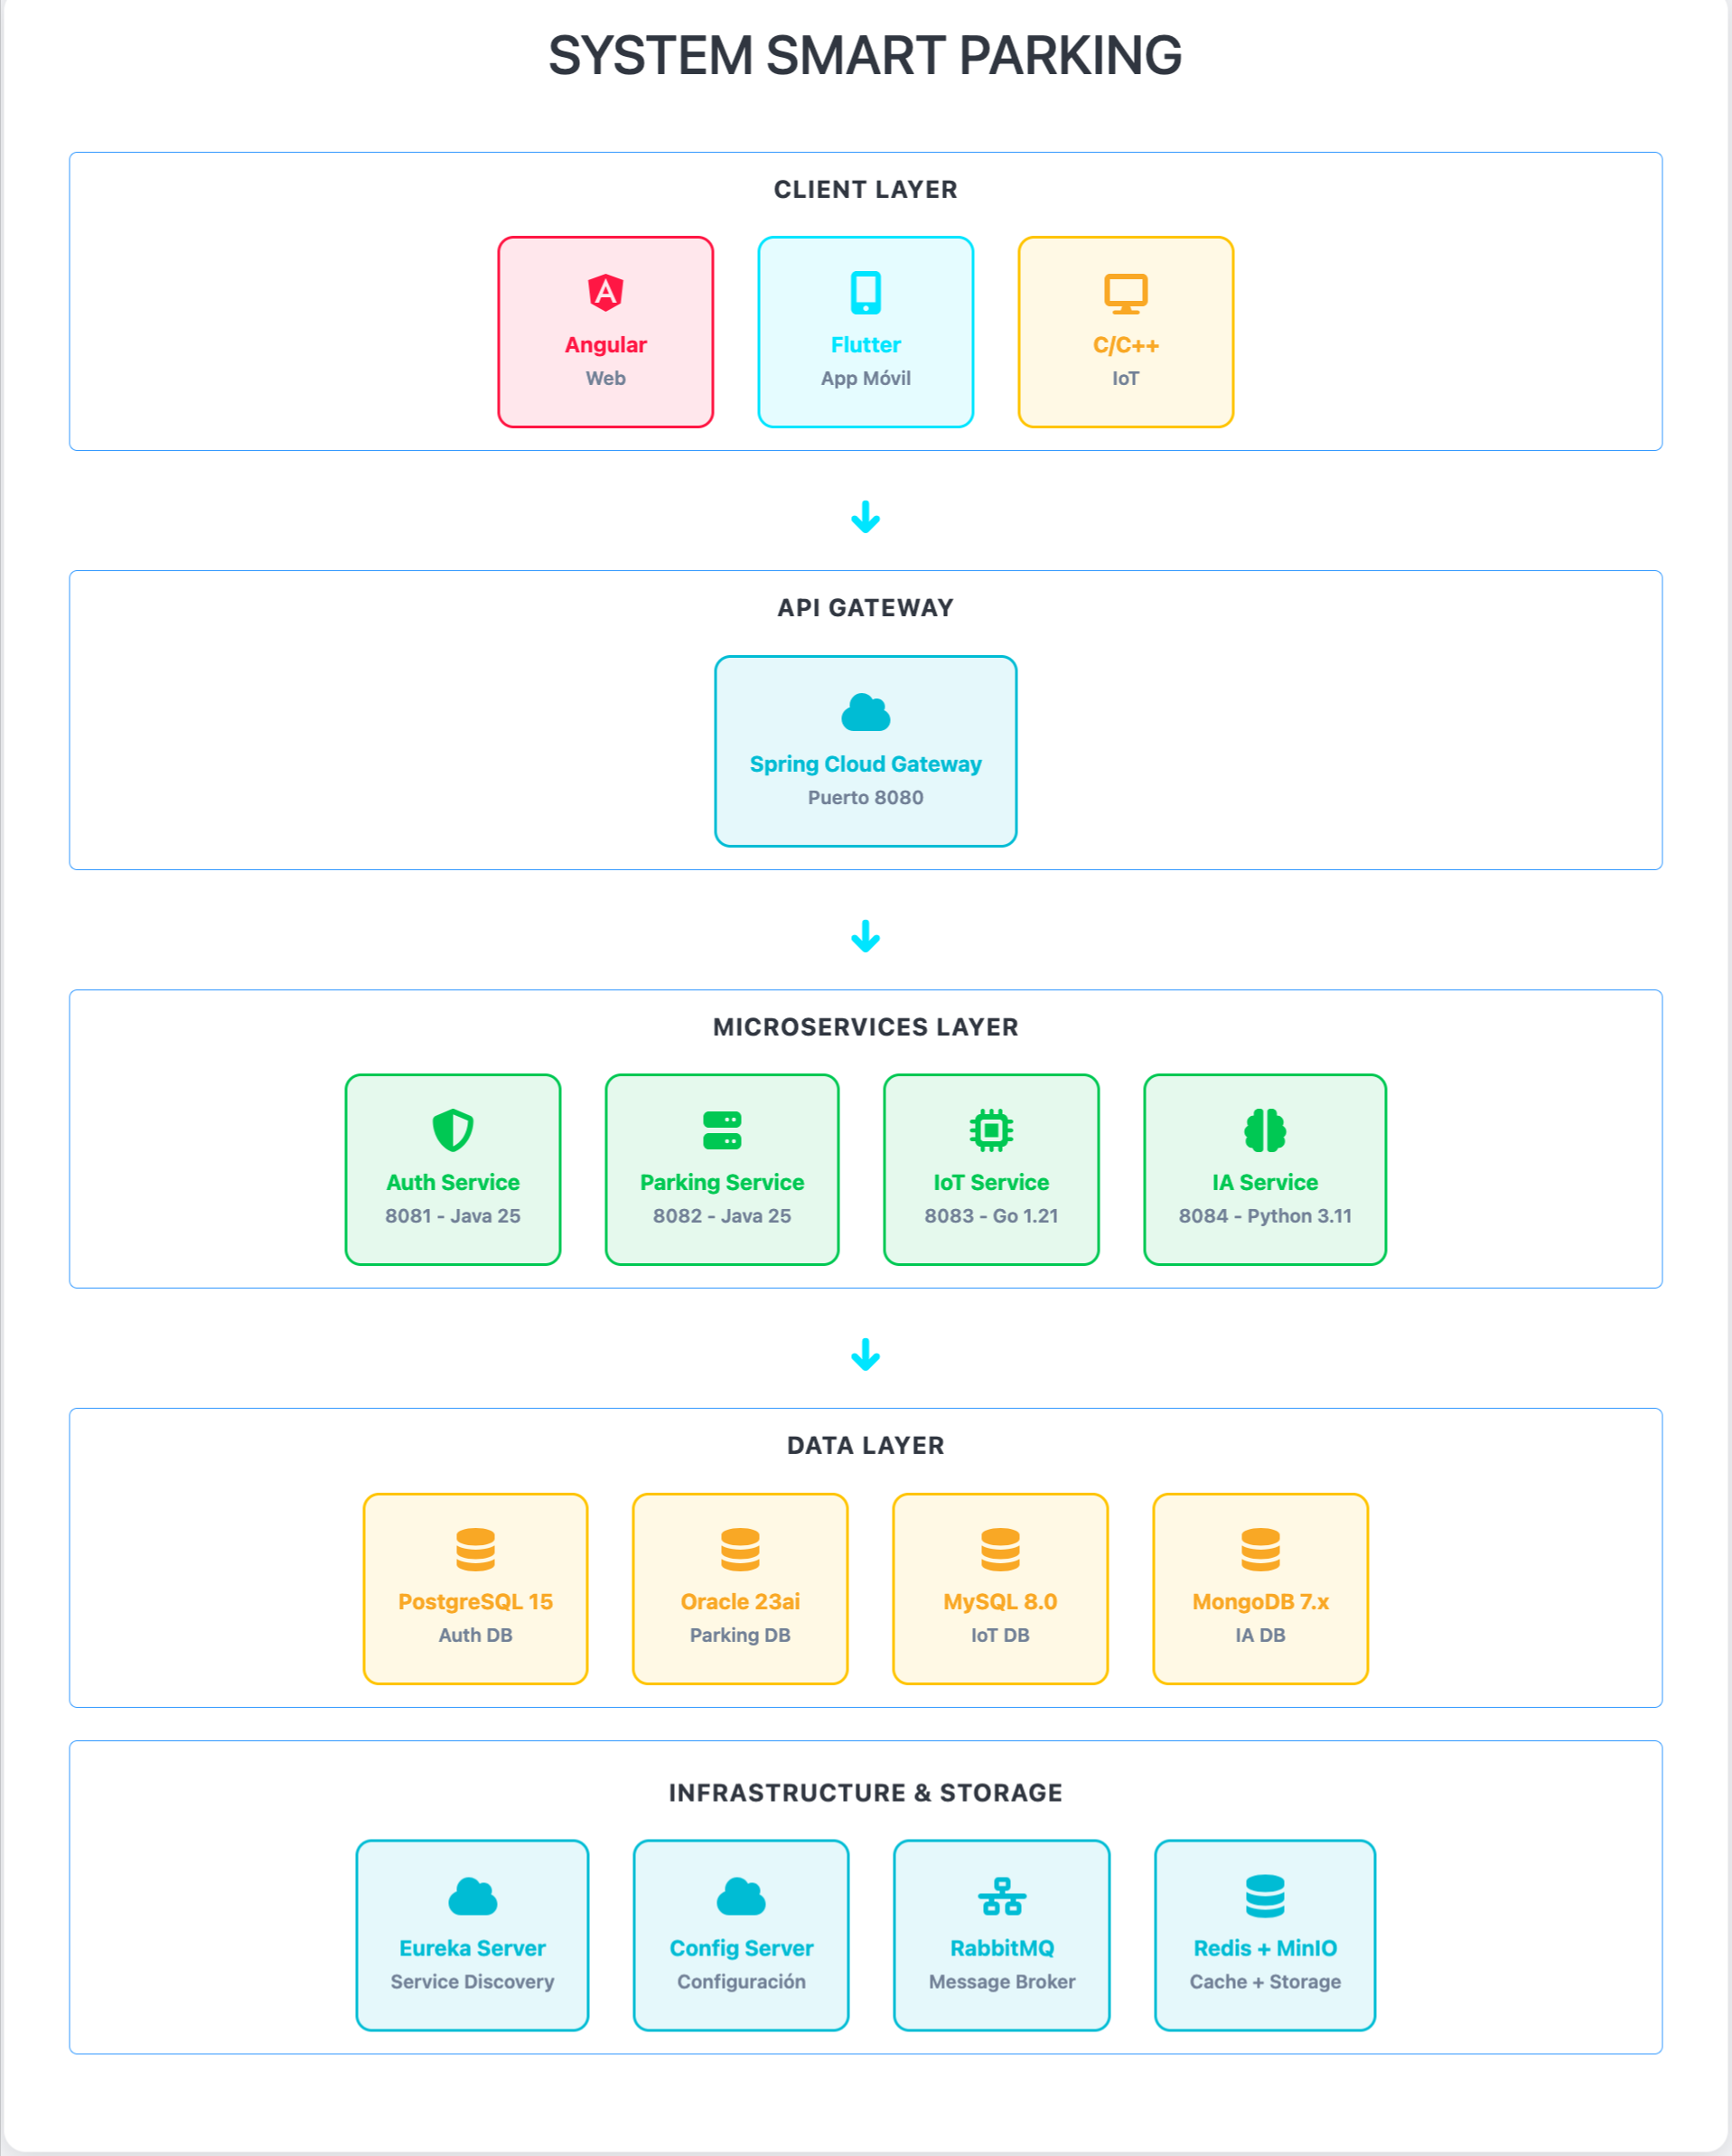
\includegraphics[width=0.80\textwidth]{architecture_smart_parking_system.png}
	
	\begin{flushleft}
		\setlength{\parskip}{0pt}
		\small \textit{Nota.} El diagrama técnico de la solución describe la arquitectura del prototipo. \\ Fuente: Elaboración propia.
	\end{flushleft}
\end{figure}

\end{document}